
%\documentclass[11pts,a4paper,amsmath,amssymb,floatfix]{article}%{report}%{book}
\documentclass[12pts,a4paper,amsmath,amssymb,floatfix]{article}%{report}%{book}
\usepackage{graphicx,wrapfig}% Include figure files
%\usepackage{dcolumn,enumerate}% Align table columns on decimal point
\usepackage{enumerate,enumitem}% Align table columns on decimal point
\usepackage{bm,dpfloat}% bold math
\usepackage[pdftex,bookmarks,colorlinks=true,urlcolor=rltblue,citecolor=blue]{hyperref}
\usepackage{amsfonts,amsmath,amssymb,stmaryrd,indentfirst}
\usepackage{times,psfrag}
\usepackage{natbib}
\usepackage{color}
\usepackage{units}
\usepackage{rotating}
\usepackage{multirow}

\usepackage{pifont}
\usepackage{subfigure}
\usepackage{subeqnarray}
\usepackage{ifthen}

\usepackage{supertabular}
\usepackage{moreverb}
\usepackage{fancyvrb}
\usepackage{listings}
\usepackage{palatino}
%\usepackage{doi}
\usepackage{longtable}
\usepackage{float}
\usepackage{perpage}
\MakeSorted{figure}
%\usepackage{pdflscape}

\definecolor{rltblue}{rgb}{0,0,0.75}


%\usepackage{natbib}
\usepackage{fancyhdr} %%%%
\pagestyle{fancy}%%%%
% with this we ensure that the chapter and section
% headings are in lowercase
%%%%\renewcommand{\chaptermark}[1]{\markboth{#1}{}}
\renewcommand{\sectionmark}[1]{\markright{\thesection\ #1}}
\fancyhf{} %delete the current section for header and footer
\fancyhead[LE,RO]{\bfseries\thepage}
\fancyhead[LO]{\bfseries\rightmark}
\fancyhead[RE]{\bfseries\leftmark}
\renewcommand{\headrulewidth}{0.5pt}
% make space for the rule
\fancypagestyle{plain}{%
\fancyhead{} %get rid of the headers on plain pages
\renewcommand{\headrulewidth}{0pt} % and the line
}

\def\newblock{\hskip .11em plus .33em minus .07em}
\usepackage{color}

%\usepackage{makeidx}
%\makeindex

\setlength\textwidth      {16.cm}
\setlength\textheight     {22.6cm}
\setlength\oddsidemargin  {-0.3cm}
\setlength\evensidemargin {0.3cm}

\setlength\headheight{14.49998pt} 
\setlength\topmargin{0.0cm}
\setlength\headsep{1.cm}
\setlength\footskip{1.cm}
\setlength\parskip{0pt}
\setlength\parindent{0pt}

%%%
%%% Headers and Footers
\lhead[] {\text{\small{EG3539 -- Thermodynamics 1A}}} 
%\chead[] {\text{\small{Session 2012/13}}} 
\lfoot[]{Module 01}
%\cfoot[\thepage]{\thepage}
\rfoot[\text{\small{\thepage}}]{\thepage}
\rhead[] {{\text{\small{Session 2012/13}}}}
\renewcommand{\headrulewidth}{0.8pt}

%%%
%%% space between lines
%%%
\renewcommand{\baselinestretch}{1.5}

\newenvironment{VarDescription}[1]%
  {\begin{list}{}{\renewcommand{\makelabel}[1]{\textbf{##1:}\hfil}%
    \settowidth{\labelwidth}{\textbf{#1:}}%
    \setlength{\leftmargin}{\labelwidth}\addtolength{\leftmargin}{\labelsep}}}%
  {\end{list}}

%%%%%%%%%%%%%%%%%%%%%%%%%%%%%%%%%%%%%%%%%%%
%%%%%%                              %%%%%%%
%%%%%%      NOTATION SECTION        %%%%%%%
%%%%%%                              %%%%%%%
%%%%%%%%%%%%%%%%%%%%%%%%%%%%%%%%%%%%%%%%%%%

% Text abbreviations.
\newcommand{\ie}{{\em{i.e., }}}
\newcommand{\eg}{{\em{e.g., }}}
\newcommand{\cf}{{\em{cf., }}}
\newcommand{\wrt}{with respect to}
\newcommand{\lhs}{left hand side}
\newcommand{\rhs}{right hand side}
% Commands definining mathematical notation.

% This is for quantities which are physically vectors.
\renewcommand{\vec}[1]{{\mbox{\boldmath$#1$}}}
% Physical rank 2 tensors
\newcommand{\tensor}[1]{\overline{\overline{#1}}}
% This is for vectors formed of the value of a quantity at each node.
\newcommand{\dvec}[1]{\underline{#1}}
% This is for matrices in the discrete system.
\newcommand{\mat}[1]{\mathrm{#1}}


\DeclareMathOperator{\sgn}{sgn}
\newtheorem{thm}{Theorem}[section]
\newtheorem{lemma}[thm]{Lemma}

%\newcommand\qed{\hfill\mbox{$\Box$}}
\newcommand{\re}{{\mathrm{I}\hspace{-0.2em}\mathrm{R}}}
\newcommand{\inner}[2]{\langle#1,#2\rangle}
\renewcommand\leq{\leqslant}
\renewcommand\geq{\geqslant}
\renewcommand\le{\leqslant}
\renewcommand\ge{\geqslant}
\renewcommand\epsilon{\varepsilon}
\newcommand\eps{\varepsilon}
\renewcommand\phi{\varphi}
\newcommand{\bmF}{\vec{F}}
\newcommand{\bmphi}{\vec{\phi}}
\newcommand{\bmn}{\vec{n}}
\newcommand{\bmns}{{\textrm{\scriptsize{\boldmath $n$}}}}
\newcommand{\bmi}{\vec{i}}
\newcommand{\bmj}{\vec{j}}
\newcommand{\bmk}{\vec{k}}
\newcommand{\bmx}{\vec{x}}
\newcommand{\bmu}{\vec{u}}
\newcommand{\bmv}{\vec{v}}
\newcommand{\bmr}{\vec{r}}
\newcommand{\bma}{\vec{a}}
\newcommand{\bmg}{\vec{g}}
\newcommand{\bmU}{\vec{U}}
\newcommand{\bmI}{\vec{I}}
\newcommand{\bmq}{\vec{q}}
\newcommand{\bmT}{\vec{T}}
\newcommand{\bmM}{\vec{M}}
\newcommand{\bmtau}{\vec{\tau}}
\newcommand{\bmOmega}{\vec{\Omega}}
\newcommand{\pp}{\partial}
\newcommand{\kaptens}{\tensor{\kappa}}
\newcommand{\tautens}{\tensor{\tau}}
\newcommand{\sigtens}{\tensor{\sigma}}
\newcommand{\etens}{\tensor{\dot\epsilon}}
\newcommand{\ktens}{\tensor{k}}
\newcommand{\half}{{\textstyle \frac{1}{2}}}
\newcommand{\tote}{E}
\newcommand{\inte}{e}
\newcommand{\strt}{\dot\epsilon}
\newcommand{\modu}{|\bmu|}
% Derivatives
\renewcommand{\d}{\mathrm{d}}
\newcommand{\D}{\mathrm{D}}
\newcommand{\ddx}[2][x]{\frac{\d#2}{\d#1}}
\newcommand{\ddxx}[2][x]{\frac{\d^2#2}{\d#1^2}}
\newcommand{\ddt}[2][t]{\frac{\d#2}{\d#1}}
\newcommand{\ddtt}[2][t]{\frac{\d^2#2}{\d#1^2}}
\newcommand{\ppx}[2][x]{\frac{\partial#2}{\partial#1}}
\newcommand{\ppxx}[2][x]{\frac{\partial^2#2}{\partial#1^2}}
\newcommand{\ppt}[2][t]{\frac{\partial#2}{\partial#1}}
\newcommand{\pptt}[2][t]{\frac{\partial^2#2}{\partial#1^2}}
\newcommand{\DDx}[2][x]{\frac{\D#2}{\D#1}}
\newcommand{\DDxx}[2][x]{\frac{\D^2#2}{\D#1^2}}
\newcommand{\DDt}[2][t]{\frac{\D#2}{\D#1}}
\newcommand{\DDtt}[2][t]{\frac{\D^2#2}{\D#1^2}}
% Norms
\newcommand{\Ltwo}{\ensuremath{L_2} }
% Basis functions
\newcommand{\Qone}{\ensuremath{Q_1} }
\newcommand{\Qtwo}{\ensuremath{Q_2} }
\newcommand{\Qthree}{\ensuremath{Q_3} }
\newcommand{\QN}{\ensuremath{Q_N} }
\newcommand{\Pzero}{\ensuremath{P_0} }
\newcommand{\Pone}{\ensuremath{P_1} }
\newcommand{\Ptwo}{\ensuremath{P_2} }
\newcommand{\Pthree}{\ensuremath{P_3} }
\newcommand{\PN}{\ensuremath{P_N} }
\newcommand{\Poo}{\ensuremath{P_1P_1} }
\newcommand{\PoDGPt}{\ensuremath{P_{-1}P_2} }

\newcommand{\metric}{\tensor{M}}
\newcommand{\configureflag}[1]{\texttt{#1}}

% Units
\newcommand{\m}[1][]{\unit[#1]{m}}
\newcommand{\km}[1][]{\unit[#1]{km}}
\newcommand{\s}[1][]{\unit[#1]{s}}
\newcommand{\invs}[1][]{\unit[#1]{s}\ensuremath{^{-1}}}
\newcommand{\ms}[1][]{\unit[#1]{m\ensuremath{\,}s\ensuremath{^{-1}}}}
\newcommand{\mss}[1][]{\unit[#1]{m\ensuremath{\,}s\ensuremath{^{-2}}}}
\newcommand{\K}[1][]{\unit[#1]{K}}
\newcommand{\PSU}[1][]{\unit[#1]{PSU}}
\newcommand{\Pa}[1][]{\unit[#1]{Pa}}
\newcommand{\kg}[1][]{\unit[#1]{kg}}
\newcommand{\rads}[1][]{\unit[#1]{rad\ensuremath{\,}s\ensuremath{^{-1}}}}
\newcommand{\kgmm}[1][]{\unit[#1]{kg\ensuremath{\,}m\ensuremath{^{-2}}}}
\newcommand{\kgmmm}[1][]{\unit[#1]{kg\ensuremath{\,}m\ensuremath{^{-3}}}}
\newcommand{\Nmm}[1][]{\unit[#1]{N\ensuremath{\,}m\ensuremath{^{-2}}}}

% Dimensionless numbers
\newcommand{\dimensionless}[1]{\mathrm{#1}}
\renewcommand{\Re}{\dimensionless{Re}}
\newcommand{\Ro}{\dimensionless{Ro}}
\newcommand{\Fr}{\dimensionless{Fr}}
\newcommand{\Bu}{\dimensionless{Bu}}
\newcommand{\Ri}{\dimensionless{Ri}}
\renewcommand{\Pr}{\dimensionless{Pr}}
\newcommand{\Pe}{\dimensionless{Pe}}
\newcommand{\Ek}{\dimensionless{Ek}}
\newcommand{\Gr}{\dimensionless{Gr}}
\newcommand{\Ra}{\dimensionless{Ra}}
\newcommand{\Sh}{\dimensionless{Sh}}
\newcommand{\Sc}{\dimensionless{Sc}}


% Journals
\newcommand{\IJHMT}{{\it International Journal of Heat and Mass Transfer}}
\newcommand{\NED}{{\it Nuclear Engineering and Design}}
\newcommand{\ICHMT}{{\it International Communications in Heat and Mass Transfer}}
\newcommand{\NET}{{\it Nuclear Engineering and Technology}}
\newcommand{\HT}{{\it Heat Transfer}}   
\newcommand{\IJHT}{{\it International Journal for Heat Transfer}}

\newcommand{\frc}{\displaystyle\frac}

\newlist{ExList}{enumerate}{1}
\setlist[ExList,1]{label={\bf Example 1.} {\bf \arabic*}}

\newlist{ProbList}{enumerate}{1}
\setlist[ProbList,1]{label={\bf Problem 1.} {\bf \arabic*}}

%%%%%%%%%%%%%%%%%%%%%%%%%%%%%%%%%%%%%%%%%%%
%%%%%%                              %%%%%%%
%%%%%% END OF THE NOTATION SECTION  %%%%%%%
%%%%%%                              %%%%%%%
%%%%%%%%%%%%%%%%%%%%%%%%%%%%%%%%%%%%%%%%%%%


% Cause numbering of subsubsections. 
%\setcounter{secnumdepth}{8}
%\setcounter{tocdepth}{8}

\setcounter{secnumdepth}{4}%
\setcounter{tocdepth}{4}%

\includeonly{Appendix_01_01,Examples_01_01,Examples_01_02,Examples_01_03}

\DeclareMathAlphabet{\mathpzc}{OT1}{pzc}{m}{it}

\begin{document}


%%%
%%%  First Page
%%%

\begin{titlepage}

\begin{center}
\bigskip

\vspace{4.cm}
\begin{center}
\resizebox{80mm}{!}{
\includegraphics[clip=true]{../FigBanner/UoALarge}}
\end{center}

\vspace{3.5cm}
\bigskip

{\bf {\huge  EG3539: Thermodynamics 1A}} \\

\bigskip
{\bf {\huge Module 01: Production of Power from Heat}}\\
{\bf {\Large Examples and Problems}}
\bigskip
\vspace{5.cm}

{\bf {\Large Dr Jeff Gomes}}
\bigskip

{\bf{\Large  School of Engineering}}\\
\vspace{3cm}    

\bigskip

{\bf {\large \today}}
\end{center}


\end{titlepage}

\setcounter{page}{1}

\vfill

\pagebreak
\tableofcontents
%\begin{Large}

\section{Module 1: Production of Power from Heat}


\subsection{Review of Thermodynamics}

\begin{enumerate}

%%%
%%%
%%%
\item {\it Given  Ar at P$_{1}$ = 140 kPa, T$_{1}$ = 10$^{o}$C, V$_{1}$ = 200 liters which undergoes a polytropic compression to P$_{2}$ = 700 kPa, T$_{2}$ = 180 $^{o}$C, find Q$_{1}^{2}$.}


In order to calculate Q$_{1}^{2}$, we will need to invoke the first law,
\begin{displaymath}
U_{2} - U_{1} = Q_{1}^{2} - W_{1}^{2} 
\end{displaymath}
For ideal gases, we need to calculate $\Delta U$ (based on $\Delta T$) and we can easily compute $W_{1}^{2}$ from its definition as $\int\limits_{1}^{2}PdV$. Using the following data for noble gas {\it Ar}:
\begin{displaymath}
MW\footnote{MW: Molecular weight; R: Universal gas constant; C$_{v}$: Heat capacity at constant volume.}=39.948 kg.\left(kmole\right)^{-1}\;\;\;\; R=0.2081 kJ.\left(kg.K\right)^{-1}\;\;\;\;C_{v}=0.312 kJ.\left(kg.K\right)^{-1}
\end{displaymath}
The mass of {\it Ar} can be calculated from state 1:
\begin{displaymath}
m=\displaystyle\frac{P_{1}V_{1}}{RT_{1}}=\displaystyle\frac{ \left(140 kPa\right) \left(0.2 m^{3}\right) } { \left(0.2081 \displaystyle\frac{kJ}{kg.K}\right) \left(283.15 K\right)} = 4.75192\times 10^{-1} kg
\end{displaymath}

The volume at state 2 can be easily calculated as,
\begin{eqnarray}
&& P_{2}V_{2}=mRT_{2} \nonumber \\
&& V_{2} =\displaystyle\frac{ \left(4.75192\times 10^{-1} kg\right) \left(0.2081 \displaystyle\frac{kJ}{kg.K}\right) \left(453.15 K\right) } {700 kPa} = 6.40155 \times 10^{-2} m^{-3} \nonumber
\end{eqnarray}

For polytropic processes,
\begin{eqnarray}
&&P_{i}V_{i}^{n} = \text{constant} = C \nonumber \\
&&\displaystyle\frac{P_{1}}{P_{2}} = \left(\displaystyle\frac{V_{2}}{V_{1}}\right)^{n} \nonumber \\
&&\ln \left( \displaystyle\frac{P_{1}}{P_{2}} \right) = \ln \left(\displaystyle\frac{V_{2}}{V_{1}}\right)^{n} \nonumber \\
&& n = \displaystyle\frac{ \ln \left( \displaystyle\frac{P_{1}}{P_{2}} \right)  } { \ln \left(\displaystyle\frac{V_{2}}{V_{1}}\right) }  = 1.41279 \nonumber
\end{eqnarray}


So the work in polyprotic processes can be defined as,
\begin{eqnarray}
W_{1}^{2} = && \int\limits_{1}^{2}\displaystyle\frac{C}{V^{n}}dV = C \int\displaystyle\frac{dV}{V^{n}} \nonumber \\
           && \left.\displaystyle\frac{C}{1-n} V^{(1-n)} \right|_{1}^{2} = \displaystyle\frac{C}{1-n}  \left( V_{2}^{(1-n)}-V_{1}^{(1-n)}\right) \nonumber
\end{eqnarray}
As $C = P_{1}V_{1} = P_{2}V_{2}$,
\begin{displaymath}
W_{1}^{2} = \displaystyle\frac{P_{2}V_{2}-P_{1}V_{1}}{1-n} = -40.7251 kJ
\end{displaymath}


The work is negative $\Longrightarrow$ {\it Ar} was worked upon in compression. From the first law,
\begin{eqnarray}
&& U_{2} - U_{1} = Q_{1}^{2} - W_{1}^{2} \nonumber \\
&& Q_{1}^{2} = U_{2} - U_{1} + W_{1}^{2} \nonumber 
\end{eqnarray}
Assuming that {\it Ar} behaves like an ideal gas, \ie $u=u(T)$ $\left(\text{with }u=\displaystyle\frac{U}{m}\right)$, 
\begin{displaymath}
\displaystyle\frac{du}{dT} = C_{v}
\end{displaymath}
and hence,
\begin{eqnarray}
Q_{1}^{2} &=& mC_{v}\left(T_{2} - T_{1}\right) + W_{1}^{2} \nonumber \\
         &=& \left( 4.75192\times 10^{-1} kg \right) \left( 0.312 kJ.\left(kg.K\right)^{-1} \right) \nonumber \left( 453.15 K - 283.15 K \right) + \left( -40.7251 kJ \right) \nonumber \\
         &=& \textcolor{red}{-15.5209 kJ} \nonumber
\end{eqnarray}
The variation of heat (or heat transfer) is negative $\Longrightarrow$ heat was lost from the system although temperature increased. This is because the raise in internal energy was mainly due to work than by the heat exchanged.   

\begin{figure}[h]
\begin{center}
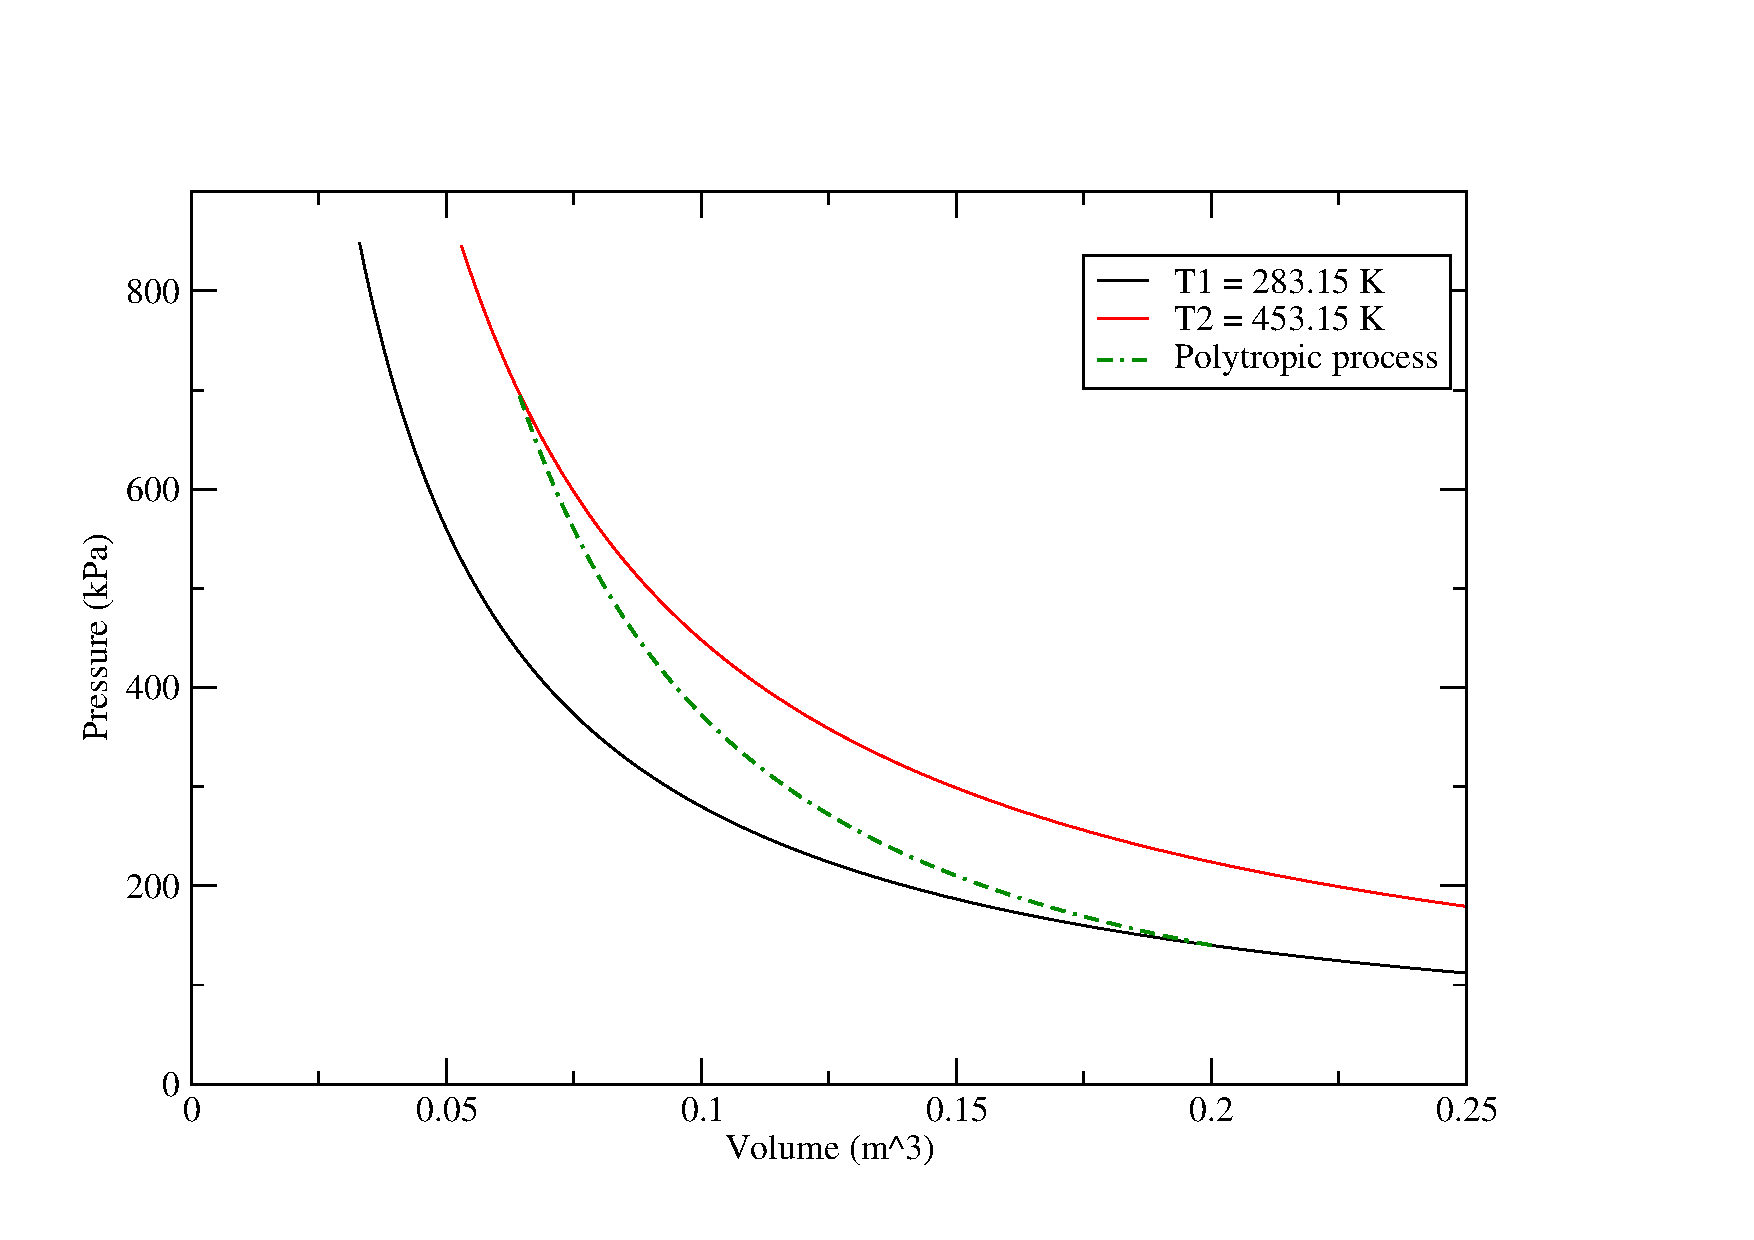
\includegraphics[width=13.0cm,height=8.0cm]{./../../ThermalEngines/Pics/example00_1}
\end{center}
\caption{Polytropic compression of {\it argonium} (green) from state 1 $\left(\text{V}_{1}=0.2 m^{3}\right)$ to 2 $\left(\text{V}_{2}=6.40\times 10^{-2}m^{3}\right)$. Ideal processes with isothermal temperature $T_{1}$ = 10 $^{o}$C (black) and $T_{2}$ = 180 $^{o}$C (red)}.
\end{figure}


%%%
%%%
%%%
\item {\it Given air (assuming ideal gas behaviour) expanding reversibly and adiabatically from $T_{1}=450 K$ and $V_{1}=3.0\times 10^{-3}m^{3}$ to the final volume, $V_{2}=5.0\times 10^{-3}m^{3}$. $T$ and $V$ relationship for constant heat capacities is represented by
\begin{displaymath}
\frc{T_{2}}{T_{1}} = \left(\frc{V_{1}}{V_{2}}\right)^{\gamma-1}
\end{displaymath}
(a) Derive a relationship between $T$ and $P$; Assuming that $C_{p}= 5.0 cal.\left(mol.K\right)^{-1}$ and $C_{v}=3.0 cal.\left(mol.K\right)^{-1}$, calculate (b) $T_{2}$, (c) the work done during the process and the (d) enthalpy change. }

The total energy change, $\Delta E$ can be split into
\begin{displaymath}
\Delta E = \Delta E_{K} + \Delta E_{P} + \Delta U = Q - W
\end{displaymath}
where $\Delta E_{K}$, $\Delta E_{P}$ and $\Delta U$ represent the change in kinetic, potential and internal energy, respectively. Assuming that the expansion process, the sum of the kinetic and potential energies of the system does not change,
\begin{displaymath}
\Delta E = \Delta U = Q - W
\end{displaymath}
or in differential form
\begin{displaymath}
dU = \delta Q - \delta W
\end{displaymath}
and all energy exchange with the surroundings are used to only change the internal energy. As the process is adiabatic ($Q=0$),
\begin{displaymath}
 dU = -\delta W = -P dV
\end{displaymath}
Since the gas is ideal, $dU=C_{v}dT = -PdV$ and,
\begin{displaymath}
V=\frc{RT}{P}
\end{displaymath}
and applying the chain rule to $V=V(T,P)$
\begin{displaymath}
dV = \frc{\partial V}{\partial T}dT + \frc{\partial V}{\partial P}dP= -\frc{RT}{P^{2}}dP + \frac{R}{P}dT
\end{displaymath}
 thus replacing $dV$,
\begin{displaymath}
C_{v}dT = - PdV = -P\left[-\frc{RT}{P^{2}}dP + \frc{R}{P}dT\right] = RT\frc{dP}{P} - RdT
\end{displaymath}
Since $C_{p}-C_{v}=R$ and replacing $C_{v}$ in the equation above,
\begin{displaymath}
C_{p}dT = RT\frc{dP}{P} \Longrightarrow \frc{dT}{T} = \frc{R}{C_{p}}\frc{dP}{P} \Longrightarrow \frc{dT}{T} = \frc{C_{p}-C_{v}}{C_{p}}\frc{dP}{P}=\left(\frc{\gamma - 1}{\gamma}\right)\frc{dP}{P}
\end{displaymath}
where $\gamma = C_{p}/C_{v}$. Integrating from state 2 to 1:
\begin{eqnarray}
&& \ln\frc{T_{2}}{T_{1}}=\left(\frc{\gamma - 1 }{\gamma}\right)\ln\frc{P_{2}}{P_{1}} \;\;\; \text{or} \nonumber \\
&& \textcolor{red}{\frc{T_{2}}{T_{1}} = \left(\frc{P_{2}}{P_{1}}\right)^{\frc{\gamma-1}{\gamma}}} \nonumber 
\end{eqnarray}

\medskip

Temperature, $T_{2}$ is obtained from 
\begin{eqnarray}
&& \frc{T_{2}}{T_{1}} = \left(\frc{V_{1}}{V_{2}}\right)^{\gamma - 1} \nonumber \\
&& T_{2} = T_{1} \left(\frc{V_{1}}{V_{2}}\right)^{\gamma - 1 } = (450\;K)\left[\frac{3.0\times 10^{-3}\;\;m^{3}}{5.0\times 10^{-3}\;\;m^{3}}\right]^{\left(\frc{5.0\;cal.\left(mol.K\right)^{-1} }{3.0\; cal.\left(mol.K\right)^{-1}  }-1\right)} \nonumber \\
&& \textcolor{red}{T_{2} = 320.12 K} \nonumber
\end{eqnarray}

The work done during the process is,
\begin{eqnarray}
&& W = -\Delta U = - C_{v}\Delta T = \left[ -3.0\; cal.\left(mol.K\right)^{-1} \right] \left( 320 - 450 \;\;K\right) \nonumber \\
&& \textcolor{red}{W = 390 \frc{cal}{mol} = 1632.85 \frc{J}{mol}} \nonumber
\end{eqnarray}
$W>0$ indicates that in the expansion process, work is done by the system. The enthalpy change of the gas can be calculated as,
\begin{eqnarray}
&& \Delta H = C_{p}\Delta T = \left[ 5.0\; cal.\left(mol.K\right)^{-1} \right] \left( 320 - 450 \;\;K\right) \nonumber \\
&& \textcolor{red}{\Delta H = -650 \frc{cal}{mol} = -2721.42 \frc{J}{mol}} \nonumber 
\end{eqnarray}


%%%
%%% Problems for the students:
%%%

%%%
%%% Problem 2.69 (Saphiro)
%%%
\item {\it Gaseous CO$_{2}$ $\left(\text{m}_{CO_{2}}=4g\right)$ is contained in a vertical piston-cylinder assembly by a piston of mass 50 kg and having a face area of 1.0$\times$10$^{-2}$m$^{2}$. The CO$_{2}$ initially occupies a volume of 5$\times$10$^{-3}$m$^{3}$ and has a specific internal energy of 657 kJ.kg$^{-1}$.  The atmosphere exerts a pressure of 100 kPa on the top of the piston. Heat transfer in the amount  of 1.95 kJ occurs slowly from the CO$_{2}$ to the surroundings, and the volume of the CO$_{2}$ decreases to 2.5$\times$10$^{-3}$m$^{3}$. Friction between the piston and the cylinder wall can be neglected. The local acceleration of gravity is 9.81 m.s$^{-2}$. For the CO$_{2}$, determine (a) the pressure in kPa and (b) the final specific internal energy in kJ.kg$^{-1}$.}

%%%
%%% Problem 2.33 (Saphiro)
%%%
\item {\it CO gas contained within a piston-cylinder assembly undergoes three processes in series:\\
       Process 1-2: expansion from p$_{1}$ = 5 bar, V$_{1}$ = 0.2 m$^{3}$ to V$_{2}$ = 1.0 m$^{3}$, during which the pressure-volume relationship is pV = constant.\\
       Process 2-3: constant volume heating from state 2 to state 3, where p$_{3}$ = 5 bar.\\
       Process 3-1: constant pressure compression to the initial state.\\
       Sketch the processes in series on p-V coordinates and evaluate the work for each process, in kJ.}

%%%
%%% Problem 2.61 (Saphiro)
%%%
\item {\it One kg of Refrigerant 22. initially at p$_{1}$ = 0.9 MPa, u$_{1}$ = 232.92 kJ/kg, is contained within a rigid closed tank The tank is fitted with a paddle wheel that transfers energy to the refrigerant at a constant rate of 0.1 kW. Heat transfer from the refrigerant to its surroundings occurs at a rate Kt, in kW, where K is a constant (in kW/min) and t is time (in min).  After 20 minutes of stirring the refrigerant is at p$_{2}$ = 1.2 MPa, u$_{2}$ = 276.67 kJ/kg. No overall changes in kinetic or potential energy occur. (a) For the refrigerant, determine the work and heat transfer; (b) determine value of the constant K (in kW/min).}

%%%
%%% Problem 2.89 (Saphiro)
%%%
\item {\it A household refrigerator operating steadily and with a coefficient of performance of 2.4 removes energy from a refrigerated  space at a rate of 600 Btu/h. Evaluating electricity at $\pounds$0.08 per kW.h, determine the cost of electricity in a month when the refrigerator operates for 360 hours.}

%%%
%%% Problem 2.90 (Saphiro)
%%%
\item {\it A heat pump cycle operating at steady state receives energy by heat transfer from well water at 10$^{o}$C and discharges energy by heat transfer to a building at the rate of 1.2$\times$10$^{5}$ kJ/h. Over a period of 14 days, an electric meter records that 1490 kW.h of electricity is provided to the heat pump. These are the only energy transfers involved.  Determine (a) the amount of energy that the heat pump receives over the 14-day period from the well water by heat transfer (in kJ), and (b) the heat pump's coefficient of performance.}


%%%
%%% Problem 2.36 (S&V)
%%%
\item {\it 1 kg of air is heated reversibly at constant pressure from an initial state of 300 K and 1 bar until its volume triples. Calculate W, Q, $\Delta$U, $\Delta$H for the process. Assume for air that
\begin{displaymath}
\frc{PV}{T} = 83.14 \;\;\; \frc{\text{bar.cm}^{3}}{mol}\;\;\;\;\;\text{and}\;\;\;\;\;C_{p}=29\frc{\text{J}}{\text{mol.K}}
\end{displaymath}
}

%%%
%%% Problem 2.37 (S&V)
%%%
\item  {\it The conditions of a gas change in a steady-flow process from 20 $^{o}$C and 1000 kPa to 60 $^{o}$C and 100 kPa. Devise a reversible non-flow process (any number of steps) for accomplishing this change of state, and calculate $\Delta$U and $\Delta$H for the process on the basis of 1 mol of gas. Assume for the gas that PV/T is constant, $C_{v}$ = (5/2)R, and $C_{p}$ = (7/2)R.}

%%%
%%% Problem 5.21-24 (Saphiro)
%%%
\item {\it A reversible power cycle receives 100 kJ by hear transfer from a hot reservoir at 327 $^{o}$C and rejects 40 kJ by heat transfer to a cold reservoir at $T_{cold}$. Determine:
\begin{enumerate}
\item The thermal efficiency;
\item The temperature $T_{cold}$;
\item Maximum theoretical thermal efficiency for any power cycle operating between hot and cold reservoirs at 602 $^{o}$C and 112 $^{o}$C, respecively;
\item Assuming that two power cycles -- PC$_{A}$ and PC$_{B}$, operate at the same thermal efficiency. PC$_{A}$ with hot and cold reservoir temperatures of 2000 K and 1000 K, respectively, and PC$_{B}$ with $T_{cold}$ an 500 K. Calculate $T_{hot}$.
\end{enumerate}
}

%%%
%%% Problem 5.78 (Saphiro)
%%%
\item \label{prob:5_78}{\it The pressure-volume diagram of a Carnot power cycle executed by an ideal gas with constant specific heat ratio $\kappa$ is shown in Fig. \ref{Prob_Saphiro_5.78}. Demonstrate that: (a) $V_{4}V_{2}=V_{1}V_{3}$, (b) $\frc{T_{2}}{T_{3}} = \left(\frc{P_{2}}{P_{3}}\right)^{\frc{\kappa - 1}{\kappa}}$ and (c) $\frc{T_{2}}{T_{3}}=\left(\frc{V_{3}}{V_{2}}\right)^{\kappa - 1}$}
\begin{figure}[h]
\begin{center}
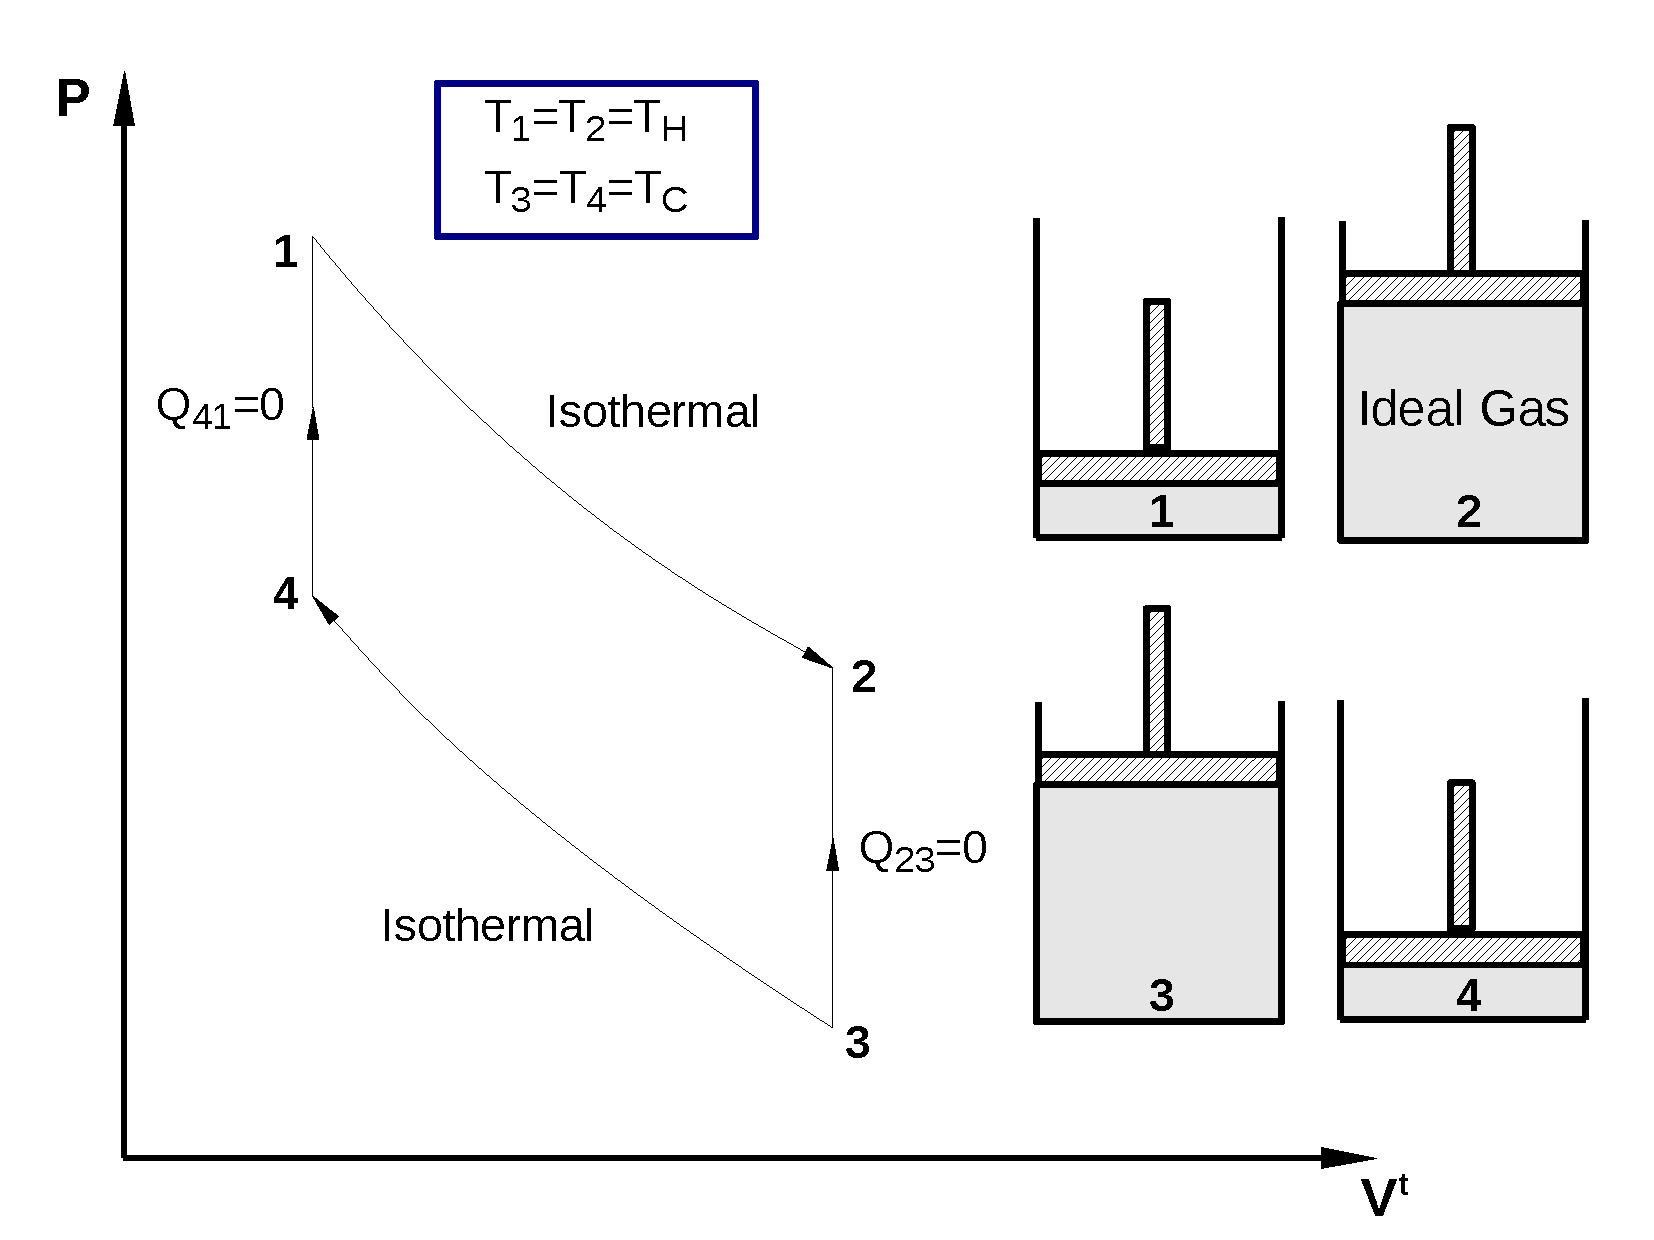
\includegraphics[width=15.cm,clip]{./../../ThermalEngines/Pics/Problem_5_78}
\caption{ \ref{prob:5_78}}
\label{Prob_Saphiro_5.78}
\end{center}
\end{figure}

%%%
%%% Problem 5.86 (Saphiro)
%%%
\item {\it A reversible refrigeration cycle $A$ and an irreversible refrigeration cycle $B$ operate between the same two reservoirs and each removes $Q_{c}$ from the cold reservoir. The net work input required by $A$ is $W_{A}$, while the net work input for $B$ is $W_{B}$. The reversible cycle discharges $Q_{H}$ to the hot reservoir, while the irreversible cycle discharges $Q^{\prime}_{H}$.  Using the Clausius inequality,, 
\begin{equation}
\oint\left(\frc{\delta Q}{T}\right) = - \sigma_{\text{cycle}} \label{eqn_clausius}
\end{equation}
show that $W_{B} > W_{A}$ and $Q^{\prime}_{H}>Q_{H}$. Using Eqn. \ref{eqn_clausius}, complete the following involving reversible and irreversible cycles:
\begin{enumerate}
\item Reversible and irreversible power cycles each discharge energy $Q_{C}$ to cold reservoir at temperature $T_{C}$ and receive energy $Q_{H}$ from hot reservoirs at temperatures $T_{H}$ and $T^{\prime}_{H}$, respectively. There are no other heat transfers in the system. Show that $T^{\prime}_{H}>T_{H}$.
\item Reversible and irreversible refrigeration cycles each discharge energy $Q_{H}$ to a hot reservoir at temperature $T_{H}$ and receive $Q_{C}$ from cold reservoirs at temperatures $T_{C}$ and $T^{\prime}_{C}$, respectively. There are no other heat transfer. Show that $T^{\prime}_{C}>T_{C}$.
\item Reversible and irreversible heat pump cycles each receive energy $Q_{C}$ from a cold reservoir at temperature $T_{C}$ and discharge energy $Q_{H}$ to hot reservoirs at temperatures $T_{H}$ and $T^{\prime}_{H}$, respectively. There are no other heat transfers. Show that $T^{\prime}_{H}<T_{H}$. 
\end{enumerate}
}

%%%
%%% Problem 5.7 (SM&VN)
%%%
\item {\it Large quantities of liquefied natural gas (LNG) are shipped by ocean tanker. At the unloading port provision is made for vaporisation of the LNG so that it may be delivered to pipelines as gas. The LNG arrives in the tanker at atmospheric pressure and 113.7 K, and represents a possible heat sink for use as the cold reservoir of a heat engine. For unloading of LNG as a vapour at the rate of 9000 $m^{3}.s^{-1}$, as measured at 298.15 K and 1.0133 bar, and assuming the availability of an adequate heat source at 303.15 K, what is the maximum possible power obtainable and what is the rate of heat transfer from the heat source? Assume that LNG at 298.15 K and 1.0133 bar is an ideal gas with the molar mass of 17. Also assume that the LNG vaporises only, absorbing only its latent heat of 512 kJ/kg at 113.7 K.}


%%%
%%% Problem 5.17 (SM&VN)
%%%
\item {\it A Carnot engine operates between temperature levels of 600 K and 300 K. It drives a Carnot refrigerator, which provides cooling at 250 K and discards heat at 300 K. Determine a numerical value for the ratio of heat extracted by the refrigerator ($\lq$cooling load') to the heat delivered to the engine ($\lq$heating load').}

%%%
%%% Problem 5.44 (SM&VN)
%%%
\item {\it A nuclear power plant generates 750 MW; the reactor temperature is 588.15 K and a river with water temperature of 293.15 K is available to provide system cooling. (a) What is the maximum possible thermal efficiency of the plant, and what is the minimum rate at which heat must be discarded to the river? (b)  If the actual thermal efficiency of the plant is 60$\%$ of the maximum, at what rate must heat be discarded to the river, and what is the temperature rise of the river if it has a flow rate of 165 $m^{3}/s$?}

%%%
%%% Problem 5.43 (SM&VN)
%%%
\item {\it Heat in the amount of 150 kJ is transferred directly from a hot reservoir at $T_{H} = 550 K$
to two cooler reservoirs at $T_{1} = 350 K$ and $T_{2} = 250 K$. The surroundings temperature is T, = 300 K. If the heat transferred to the reservoir at $T_{1}$ is half that transferred to the reservoir at $T_{2}$, calculate: (a) The entropy generation (in kJ/K); (b) The lost work ; (c) How could the process be made reversible?}


%%%
%%% Problem 8.3 (Power Lectures Notes)
%%%
\item {\it Given saturated ammonia vapour at $P_{1} = 200 kPa$ compressed by a piston to $P_{2} = 1.6 MPa$ in a
reversible adiabatic process, (a) find the work done per unit mass; (b) sketch the T-s and P-v diagrams.}

%%%
%%% Problem 8.5 (Power Lectures Notes)
%%%
\item {\it Given the enthalpy change (in water-steam thermodynamic table), calculate the entropy change for water going from saturated liquid to saturated vapour along a T = 100 ◦C isotherm.}


%%%
%%% Problem -- Callen
%%%
\item {\it Derive the Maxwell relations below,
\begin{displaymath}
%
 \left(\frac{\partial T}{\partial V}\right)_{s} = -\left(\frc{\partial P}{\partial s}\right)_{V} \;\;\;\;
%
 \left(\frc{\partial T}{\partial P}\right)_{s} = \left(\frac{\partial V}{\partial s}\right)_{P} \;\;\;\;
%
 \left(\frc{\partial P}{\partial T}\right)_{V} = \left(\frac{\partial s}{\partial V}\right)_{T} \;\;\;\;
%
  \left(\frac{\partial V}{\partial T}\right)_{P} = -\left(\frc{\partial s}{\partial P}\right)_{T} \;\;\;\; 
\end{displaymath}
from the fundamental thermodynamic equations,
\begin{eqnarray}
&& du = - PdV + Tds \nonumber \\ 
&& dh =   Tds + VdP \nonumber \\
&& df = - PdV - sdT \nonumber \\
&& dg = - VdP - sdT \nonumber
\end{eqnarray}}

\end{enumerate}

%\end{Large}

\pagebreak

\subsection{Carnot and Rankine Steam Cycles}


\begin{enumerate}

%%%
%%%
%%%
\item {\it In a turbine, steam at 20 bar, 360$^{o}$C is expanded to 0.08 bar. The steam is condensed into saturated liquid water. The pump feeds the water back into the boiler. Assume ideal processes, calculate the net work per kg of steam and the cycle efficiency.}\label{Example_01_01}

\begin{figure}[h]
\begin{center}
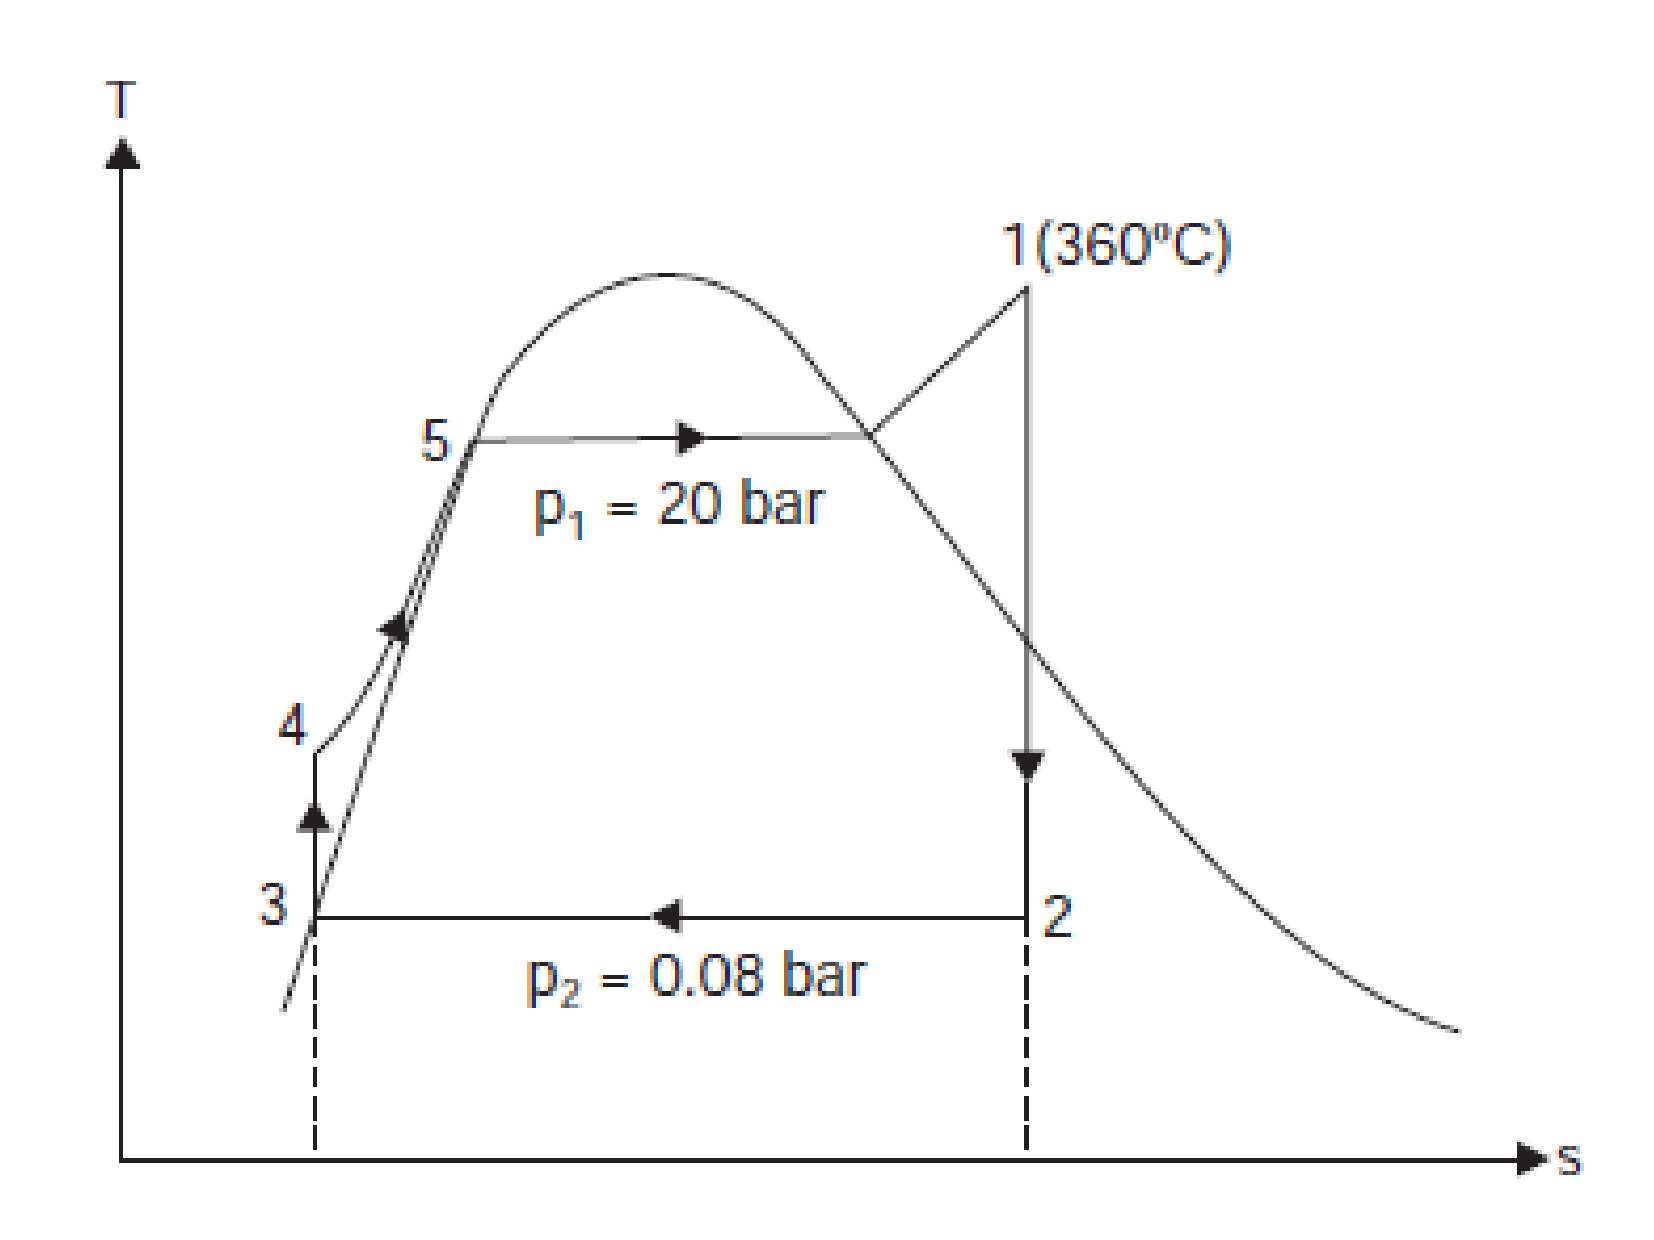
\includegraphics[width=13.0cm,height=8.0cm]{./../../ThermalEngines/Pics/example01_01}
\end{center}
\caption{Carnot and Rankine Cycles: Ts diagram -- Example \ref{Example_01_01}.}
\label{Example01_01:Pic1}
\end{figure}

As the process {\it 1-2} is isentropic (Fig. \ref{Example01_01:Pic1}), $s_{1}=s_{2}$ and using the data in Table \ref{Example01_01:Table1},
\begin{eqnarray}
&& 6.9917 = s_{f,2}+x_{2}s_{fg,2} = 0.5926 + 7.6361 x_{2} \;\; \Longrightarrow \;\; x_{2}= 0.838 \nonumber \\
&& h_{2} = h_{f,2}+ x_{2}h_{fg,2} \;\; \Longrightarrow h_{2}=2187.68\;kJ/kg \nonumber
\end{eqnarray}

\begin{center}
\begin{table}[h]
\begin{tabular}{c c c c c c c c c }
\hline
                    & $P$   & $T$ &  $h_{f}$  & $h_{fg}$ & $s_{f}$      & $s_{fg}$      & $s_{g}$        &   $v_{f}$ \\
                    & (bar) & (K) &  (kJ/kg) &  (kJ/kg) & (kJ/(kg.K)) & (kJ/(kg.K))   & (kJ/(kg.K))   &$\left(m^{3}/kg\right)$ \\
\hline
{\it Boiler}        & 20    & 633.15& 3159.3  & --      & 6.9917      & --            & --             & --  \\
\hline
{\it Condenser}     & 0.08  &  --  & 173.88  & 2403.1   & 0.5926      &  7.6361       & 8.2287         & 1.008$\times$10$^{-3}$ \\
\hline
\end{tabular}
\caption{Carnot and Rankine Cycles: Steam tables -- Example \ref{Example_01_01}.}
\label{Example01_01:Table1}
\end{table}
\end{center}

The net work $\left(W_{\text{net}}\right)$ is calculated from, $W_{\text{net}}=W_{\text{turbine}}-W_{\text{pump}}$. The work required by the pump is
\begin{eqnarray}
&& W_{\text{pump}}=h_{f,4}-h_{f,3}=v_{f,2}\left(P_{1}-P_{2}\right) = 1.008\times 10^{-3} \left[\frc{m^{3}}{kg}\right] \times (20-0.08) [bar] \times \left[\frc{100\;kJ/kg}{m^{3}.bar/kg}\right] = 2.008\; kJ/kg \nonumber \\
&& h_{f,4} = 2.008+h_{f,2}=175.89\;kJ/kg\nonumber
\end{eqnarray}
And the work produced by the tubine is defined as
\begin{displaymath}
W_{\text{turbine}}=h_{1}-h_{2} = 3159.3-2187.68= 971.62 \; kJ/kg
\end{displaymath}

And the net work is
\begin{eqnarray}
&& W_{\text{net}}=W_{\text{turbine}}-W_{\text{pump}} = 971.62-2.008 \nonumber \\
&& \textcolor{red}{W_{\text{net}}=969.61\frc{kJ}{kg}} \nonumber
\end{eqnarray}

The efficiency of the cycle is obtained by the relationship $\eta_{\text{cycle}}=\frc{W_{\text{net}}}{Q_{1}}$. The heat added into the boiler $\left(Q_{1}\right)$ is given by,
\begin{displaymath}
Q_{1}=h_{1}-h_{f,4}=3159.3-175.89=2983.41\;kJ/kg
\end{displaymath}
and the efficiency is
\begin{displaymath}
\textcolor{red}{\eta_{\text{cycle}}=\frc{969.61}{2983.41}=0.325\text{ or } 32.5\%}
\end{displaymath}


%%%
%%%
%%%
\item {\it A Rankine cycle operates between pressures of 80 and 0.1 bar and the maximum temperature is 873.15 K. Assuming that the steam turbine and condensate pump efficiencies are 90$\%$ and 80$\%$, respectively, calculate the specific work and thermal efficiency.}\label{Example_01_02}

From the saturated water and steam tables:

\begin{center}
\begin{table}[h]
\begin{tabular}{||c|c|c c|c c c|c c c||} 
\hline\hline
{\bf P (bar)} & {\bf T (K)} & \multicolumn{2}{|c|}{{\bf Specific Volume $\left(m^{3}/kg\right)$}} & \multicolumn{3}{|c|}{{\bf Specific Enthalpy (kJ/kg)}} & \multicolumn{3}{|c||}{{\bf Specific Entropy (kJ/(kg.K)}}  \\
\hline
              &             &  $v_{f}$                  &    $v_{g}$                              &  $h_{f}$    &  $h_{fg}$  &   $h_{g}$                 &  $s_{f}$  &  $s_{fg}$    &  $s_{g}$  \\
\hline\hline
0.1           & 318.99      &1.0103$\times$10$^{-3}$    & 0.1468$\times$10$^{2}$                  & 191.9   & 2392.3    & 2584.2              & 0.6488 & 7.5006  & 8.1494 \\
80            & 568.25      &1.385$\times$10$^{-3}$     & 0.0235                                  & 1317.0 & 1440.5   & 2757.5               & 3.2073 & 2.5351  & 5.7424  \\
\hline\hline
\end{tabular}
\caption{Carnot and Rankine Cycles: From Saturated water and steam tables.}
\label{Example01_01:Table2}
\end{table}
\end{center}


\begin{table}[h]
\begin{center}
\begin{tabular}{c c r}
\multicolumn{3}{c}{Superheated Steam} \\
\hline
\multirow{3}{*}{$P=80\;bar\;,\;T= 600^{o}C$} & $v$ & 0.486 m$^{3}$/kg \\
                           & $h$ & 3642 kJ/kg \\
                           & $s$ & 7.0206 kJ/(kg.K)\\
\hline
\end{tabular}
\end{center}
\caption{Carnot and Rankine Cycles: From Superheated Steam.}
\label{Example01_01:Table23}
\end{table}

Since $s_{1}=s_{2}$, the steam quality is calculated from,
\begin{eqnarray}
&& s_{2} = s_{f,2}+x_{2}s_{fg,2} \nonumber \\
&& 7.0206 =  0.6488 + 7.5006 x_{2} \nonumber \\
&& x_{2}= 0.85
\end{eqnarray}
and the enthalpy is obtained from 
\begin{displaymath}
h_{2}=h_{f,2}+x_{2}h_{fg,2} =191.9+0.85\times 2392.3 = 2225.36\; kJ/kg
\end{displaymath}
And the work


\begin{figure}[h]
\begin{center}
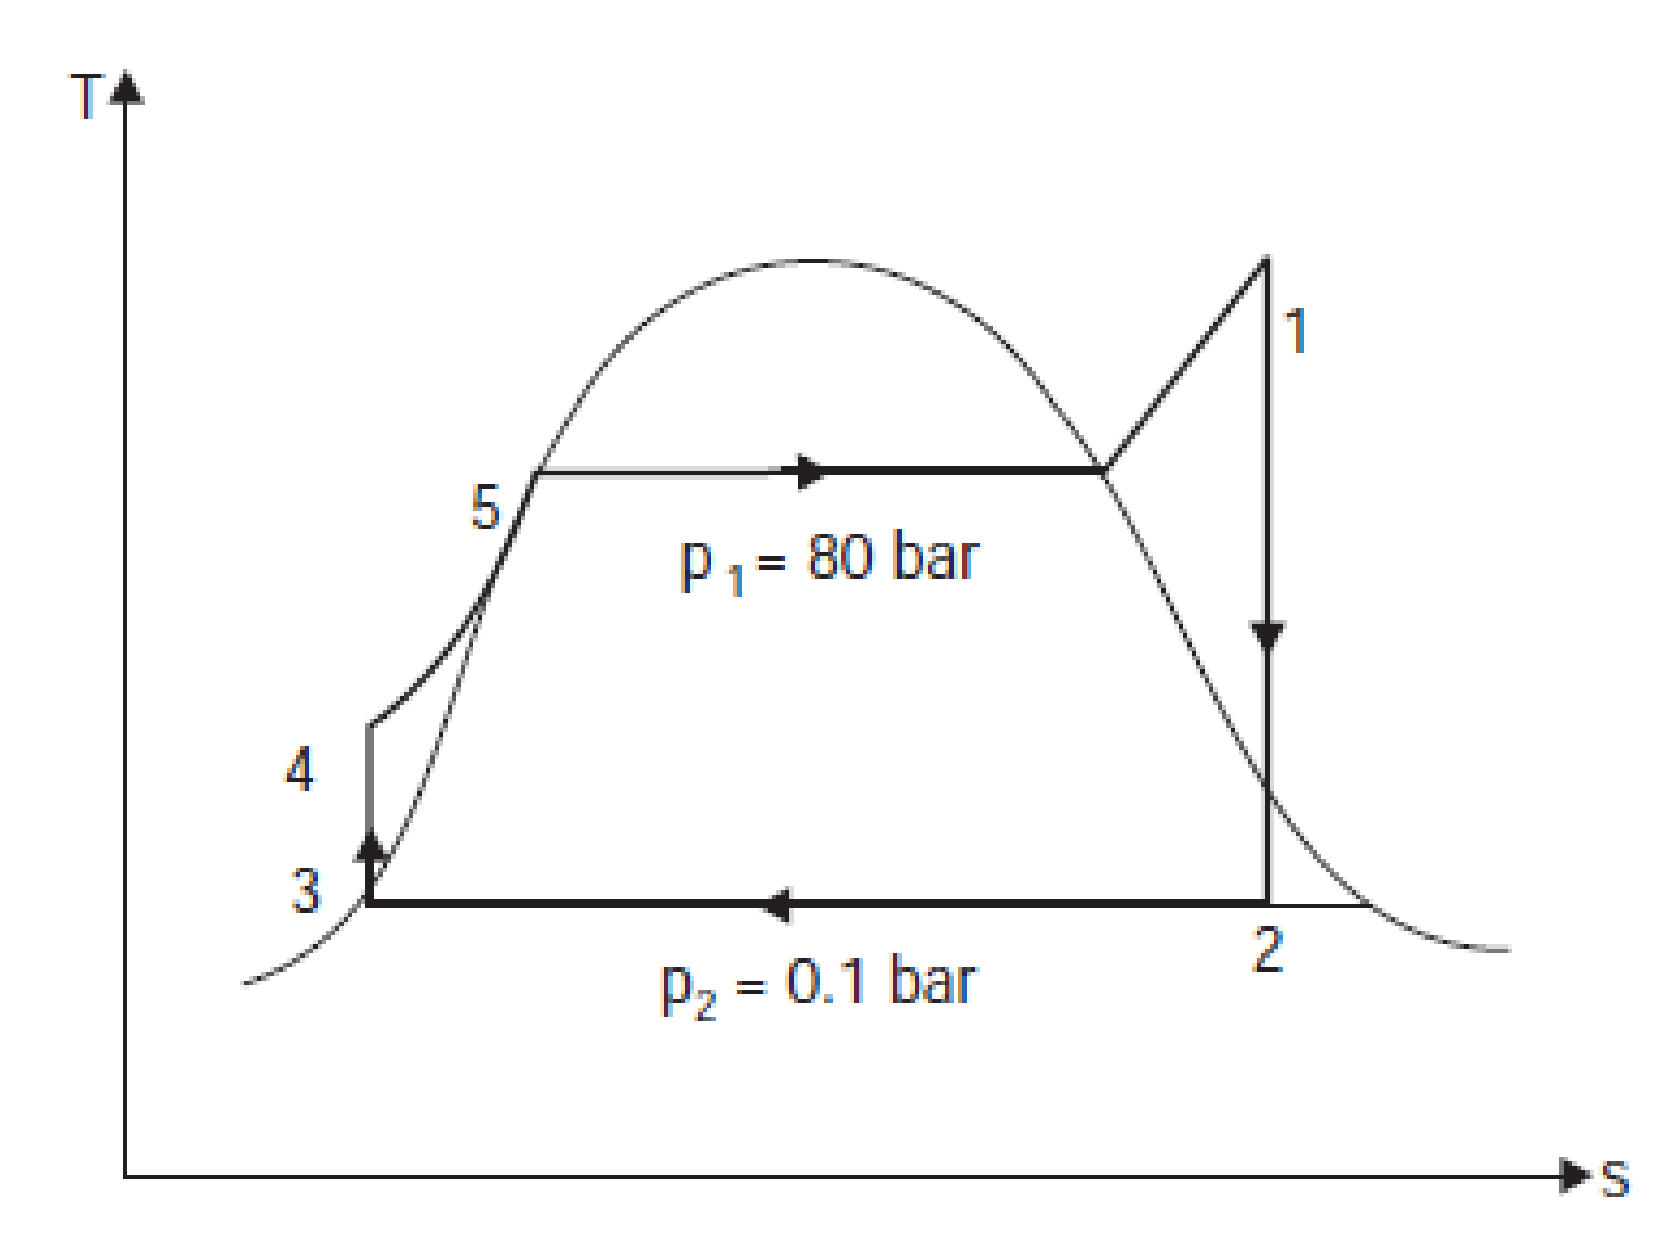
\includegraphics[width=13.0cm,height=8.0cm]{./../../ThermalEngines/Pics/example01_02}
\end{center}
\caption{Carnot and Rankine Cycles: Ts diagram -- Example \ref{Example_01_02}.}
\label{Example01_01:Pic2}
\end{figure}

%%%
%%%
%%%
\item {\it In a steam power plant operating on the Rankine cycle, steam enters the turbine at 30 bar and 623.15 K and later condensed at 0.1 bar. Calculate: (a) thermal efficiency; (b) thermal efficiency assuming that the steam is superheated to 873.15 K before entering the turbine; (c)thermal efficiency assuming that the boiler pressure is raised to 150 bar while the inlet temperature at turbine is maintained at  623.15 K.}\label{Example_01_03}


\begin{enumerate}
\item \label{example_01_03_a}The {\it Ts} diagrams of the cycle for all three cases can be seen in Fig. \ref{Example01_01:Pic3}, and the original phase states can assigned as 

\begin{tabular}{l l l l}
$P_{1}=0.1\;bar$ (saturated liquid) &  $P_{2}=30\;bar$ & $P_{3}=30\;bar$           & $P_{4}=0.1\;bar$ \\
$h_{1}=191.81\;kJ/kg$               &  $s_{2}=s_{1}$   & $T_{3}=623.15\;K$         & $s_{4}=s_{3}$ \\
$v_{1}=1.01\times 10^{-3}\;m^{3}/kg$ &                  & $h_{3}=3116.1\;kJ/kg$     &                 \\
                                    &                 & $s_{3}=6.7450\;kJ/(kg.K)$ &                 \\
\end{tabular}


\begin{figure}[h]
\begin{center}
\vbox{
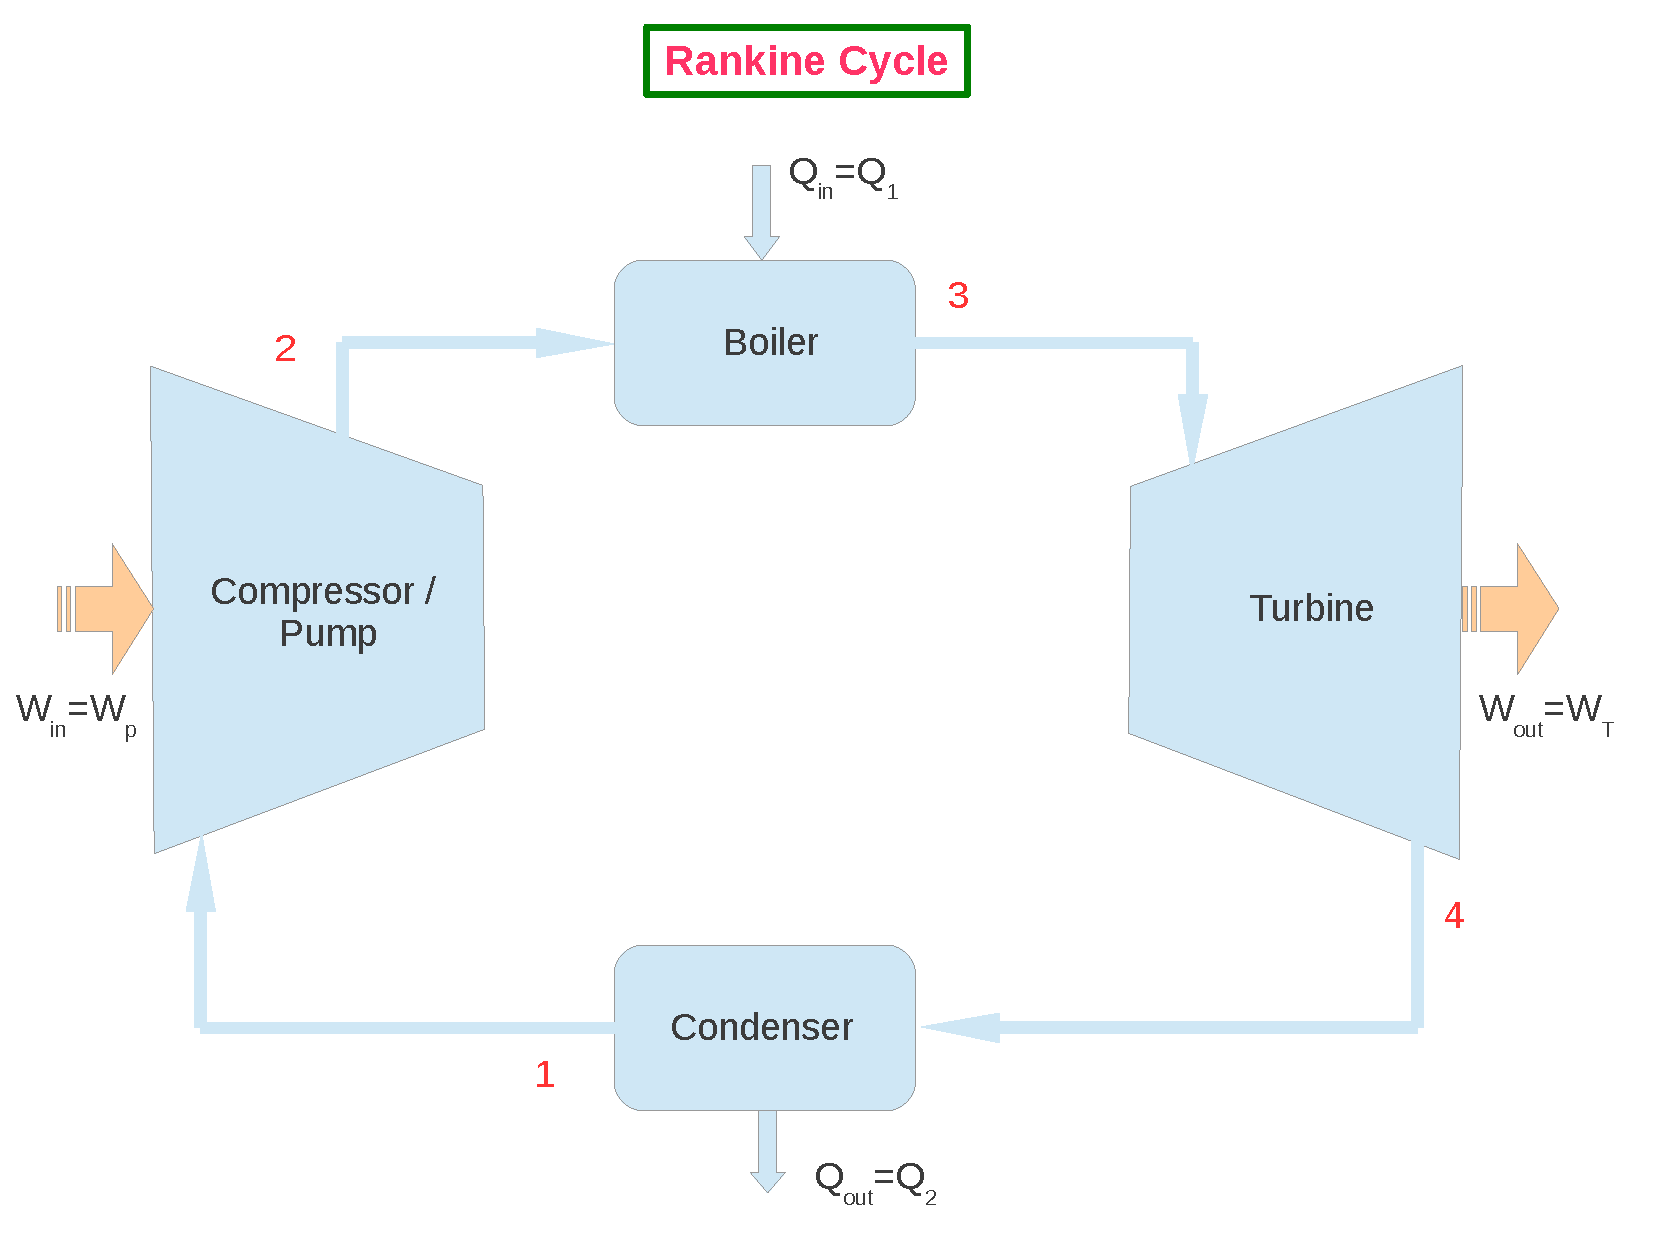
\includegraphics[width=13.0cm,height=9.0cm]{./../../ThermalEngines/Pics/Simple_Rankine_Cycle_2}
\vspace{-1.cm}
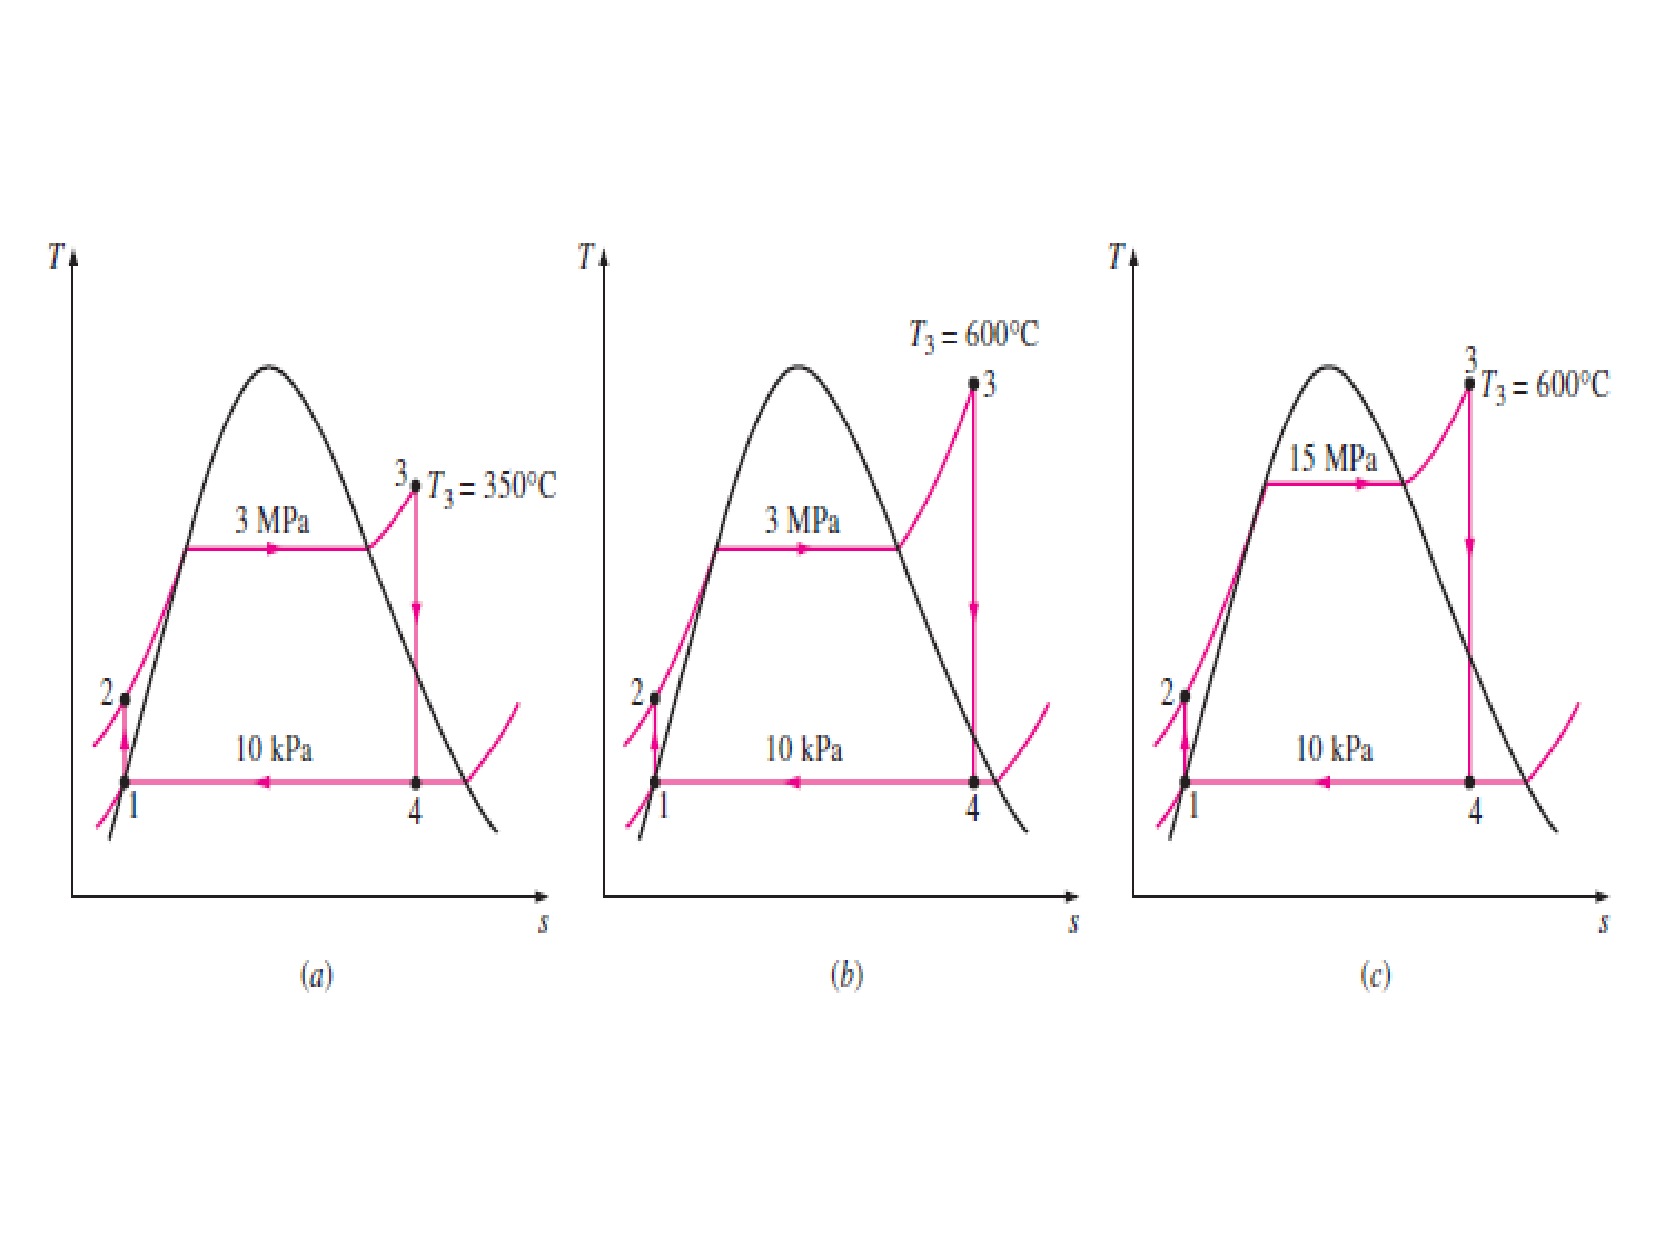
\includegraphics[width=15.0cm,height=9.0cm]{./../../ThermalEngines/Pics/example01_03}
}
\end{center}
\caption{Carnot and Rankine Cycles: Schematic of a Rankine cycle and Ts diagrams -- Example \ref{Example_01_03}.}
\label{Example01_01:Pic3}
\end{figure}

Enthalpy of the fluid leaving the pump can be calculated as
\begin{displaymath}
h_{2}=h_{1}+W_{\text{in}}
\end{displaymath}

where the pump work can be computed as
\begin{displaymath}
W_{\text{in}}=v_{1}\left(P_{2}-P_{1}\right)=3.02\;kJ/kg
\end{displaymath}
therefore the fluid's enthalpy is $h_{2}=194.83\;kJ/kg$. The fluid quality at the turbine output is (assuming isentropic process),
\begin{displaymath}
x_{4}=\frc{s_{4}-s_{f}}{s_{fg}}=\frc{6.7450-0.6492}{7.4996}=0.8128
\end{displaymath}
Thus,
\begin{eqnarray}
&& h_{4}=h_{f}+x_{4}h_{fg}=191.81+0.8128\times 2392.1=2136.1\;kJ/kg \nonumber \\
&& q_{\text{in}}=h_{3}-h_{2}=3116.1-194.83=2921.3\;kJ/kg \nonumber \\
&& q_{\text{out}}=h_{4}-h_{1}=2136.1-191.81=1944.3\;kJ/kg
\end{eqnarray}

and the cycle efficiency is given by,
\begin{displaymath}
\textcolor{blue}{\eta_{\text{(a)}}=1-\frc{q_{\text{out}}}{q_{\text{in}}} = 1 - \frc{1944.3}{2921.3} = 0.334 \text{ or } 33.4\%}
\end{displaymath}

\item \label{example_01_03_b} For this case, phase-states (1) and (2) remain the same whereas the enthapies of (2) and (4) need to be updated

\begin{tabular}{l l l l}
$P_{1}=0.1\;bar$ (saturated liquid) &  $P_{2}=30\;bar$ & $P_{3}=30\;bar$           & $P_{4}=0.1\;bar$ \\
$h_{1}=191.81\;kJ/kg$               &  $s_{2}=s_{1}$   & $T_{3}=873.15\;K$         & $s_{4}=s_{3}$ \\
$v_{1}=1.01\times 10^{-3}\;m^{3}/kg$ &                  & $h_{3}=3682.8\;kJ/kg$     &                 \\
                                    &                 & $s_{3}=7.509\;kJ/(kg.K)$ &                 \\
\end{tabular}

and using the same procedure as Example \ref{example_01_03_a}, $x_{4}=0.915$ and $h_{4}=2380.3\;kJ/kg$. Added and removed heats are
\begin{eqnarray}
&& q_{\text{in}}=h_{3}-h_{2}=3682.8-194.83=3488.0\;kJ/kg \nonumber \\
&& q_{\text{out}}=h_{4}-h_{1}=2380.3-191.81=2188.5\;kJ/kg \nonumber \\
\end{eqnarray}

and the cycle efficiency is given by,
\begin{displaymath}
\textcolor{blue}{\eta_{\text{(b)}}=1-\frc{q_{\text{out}}}{q_{\text{in}}} = 1 - \frc{2188.5}{3488.0} = 0.373 \text{ or } 37.3\%}
\end{displaymath}

The thermal efficiency increases from 33.4$\%$ to 37.3$\%$ (Table \ref{Example01_01:Table2}) as superheated steam temperature is raised from 623.15 K to 873.15 K with a smaller amount of moisture -- from 18.7$\%$ to 8.5 $\%$ (i.e., steam quality increases from 81.3$\%$ to 91.5$\%$).

\item \label{example_01_03_c} For this case, phase-state (1) remain the same but all other phase-states changes. Enthalpies are determined in a similar way as shown in Example \ref{example_01_03_a}: $h_{2}=206.95\;kJ/kg$, $h_{3}=3583.1\;kJ/kg$ and $h_{4}=2115.3\;kJ/kg$ with steam quality as $x_{4}=0.804$.  Added and removed heats then become
\begin{eqnarray}
&& q_{\text{in}}=h_{3}-h_{2}=3583.1-206.95=3376.2\;kJ/kg \nonumber \\
&& q_{\text{out}}=h_{4}-h_{1}=2115.3-191.81=1923.5\;kJ/kg \nonumber \\
\end{eqnarray}

and the cycle efficiency is given by,
\begin{displaymath}
\textcolor{blue}{\eta_{\text{(c)}}=1-\frc{q_{\text{out}}}{q_{\text{in}}} = 1 - \frc{1923.5}{3376.2} = 0.430 \text{ or } 43.0\%}
\end{displaymath}

\medskip


The thermal efficiency increases from 37.3$\%$ to 43.0 $\%$ as the boiler pressure is raised from 30 to 150 bar with constant turbine inlet temperature, 623.15 K (Table \ref{Example01_01:Table2}).

\begin{table}
\begin{center}
\begin{tabular}{c |l l l }
\hline
          &  {\bf Case (a)}      &  {\bf Case (b) }     &  {\bf Case (c) }    \\ 
\hline 
          &   $P_{3}=30\;bar$     &  $P_{3}=30\;bar$     &  $P_{3}=150\;bar$    \\
          &   $T_{3}=623.15\;K$   &  $T_{3}=673.15\;K$   &  $T_{3}=623.15\;K$   \\
          &   $P_{1}=0.1\;bar$    &  $P_{1}=0.1\;bar$    &  $P_{1}=0.1\;bar$    \\
          &   $x_{4}=0.8128$      &   $x_{4}=0.915$      &  $x_{4}=0.804$       \\
\hline
\textcolor{blue}{$\eta \left(\%\right)$} &3\textcolor{blue}{3.4} &\textcolor{blue}{37.3}& \textcolor{blue}{43.0}      \\
\end{tabular}
\end{center}
\caption{Carnot and Rankine Cycles: Improving the efficiency of Rankine cycles, Example \ref{Example_01_03}.}
\label{Example01_01:Table2}
\end{table}



\end{enumerate}

%%%
%%%  Problem 8.2 (SM&VN)
%%%

\item {\it A Carnot engine with water/steam (1 kg/s) as the working fluid operates on the cycle shown in Fig. \ref{PVTSDiags}. For $T_{1}=475\;K$ and $T_{2}=300\;K$, determine: (a) pressures at states 1, 2, 3, and 4; (b) quality $x^{\text{vapour}}$ at states 2 and 3; (c) rate of heat addition; (d) rate of heat rejection; (e) mechanical power for each of the four steps; (f) thermal efficiency $\left(\eta\right)$ of the cycle.}
   \begin{figure}[h]
    \begin{center}
     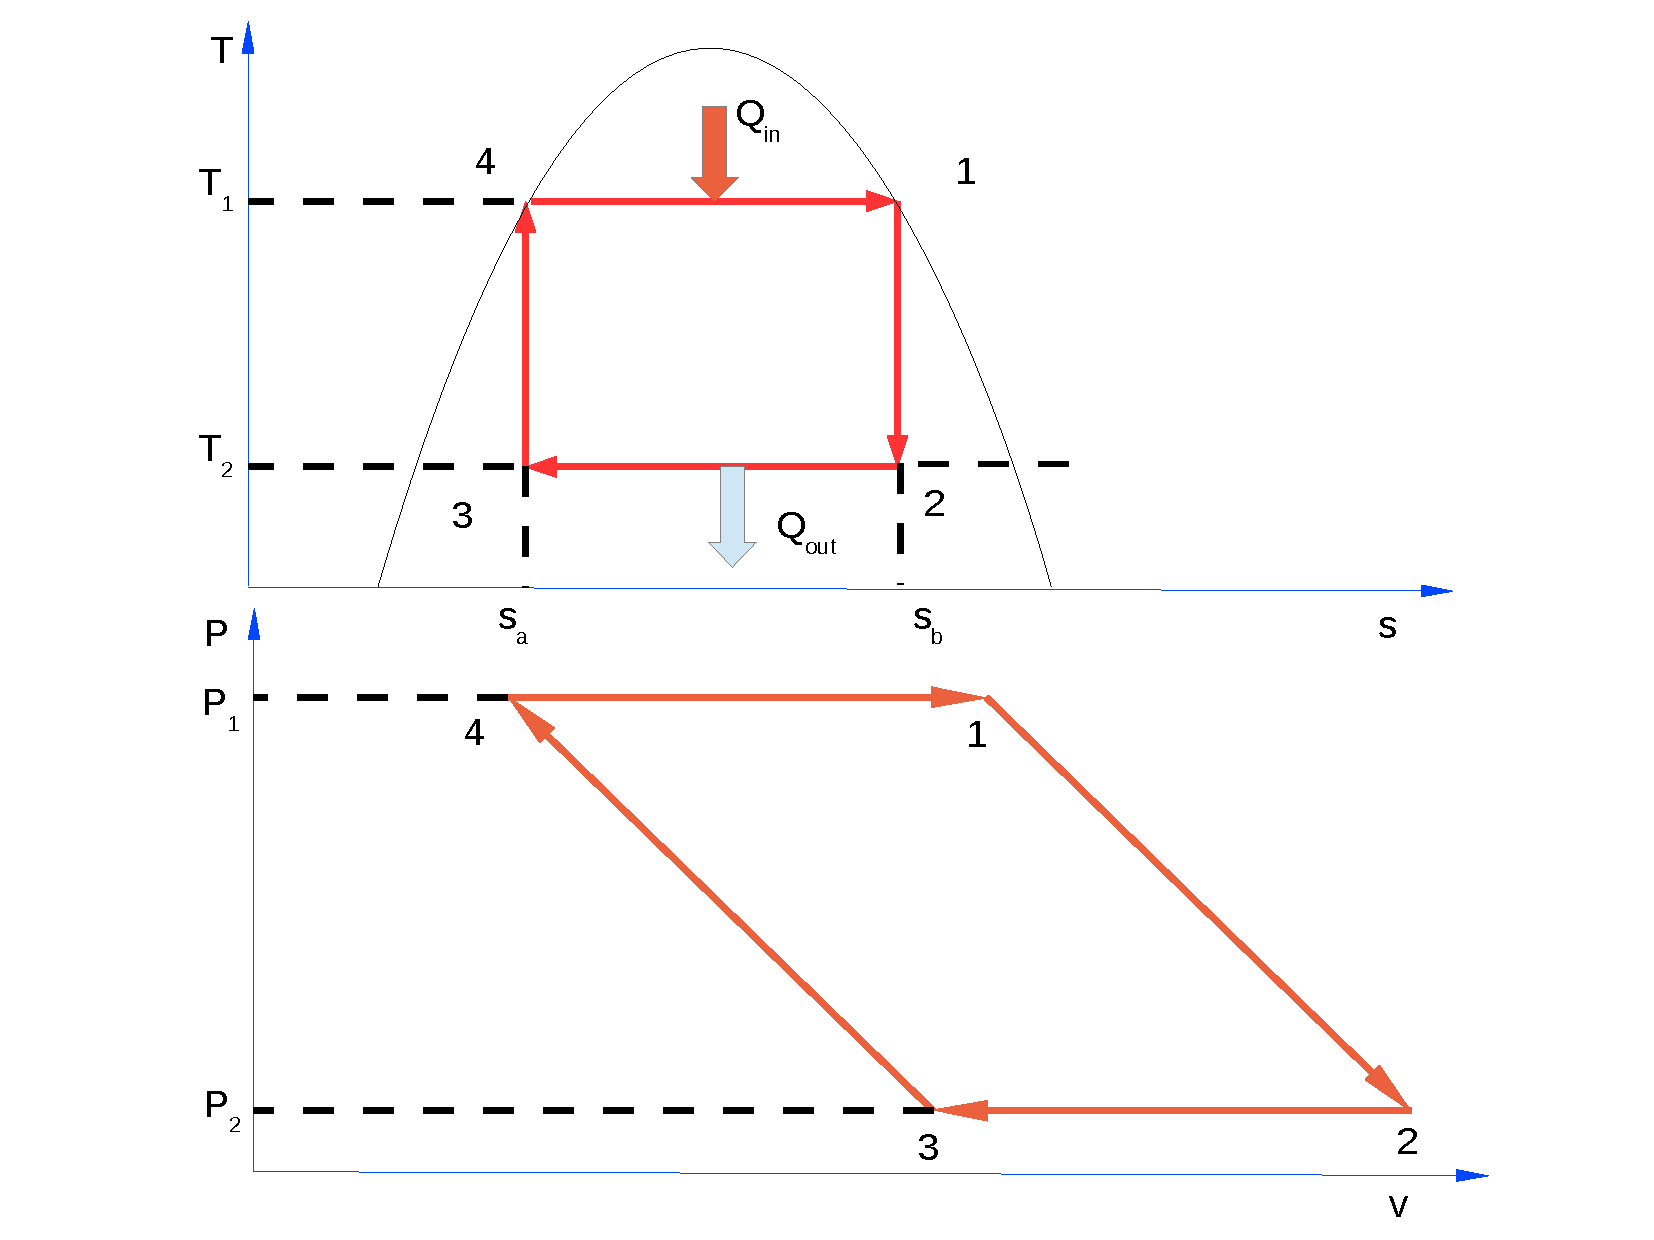
\includegraphics[width=12.cm,clip]{./../../ThermalEngines/Pics/Carnot_PV_TS}
    \end{center}
    \caption{Ts and Pv diagrams for Carnot cycle.}\label{PVTSDiags}
   \end{figure}    

%%%
%%% Problem 8.3 (SM&VN)
%%%
%\item {\it A steam power plant operates on the cycle of Fig. \ref{GenericSteamPlant}. For one of the following sets of operating conditions, determine the steam rate, the heat-transfer rates in the boiler and condenser, and the thermal efficiency of the plant.
%\begin{enumerate}
%\item P1 = P2 = 10000 kPa; T2 = 873.15 K; P3 = P4 = 10     kPa; $\eta_{\text{turbine}}$ = 0.80; $\eta_{\text{pump}}$ = 0.75; power rating = 80  MW.
%\item P1 = P2 = 7000  kPa; T2 = 823.15 K; P3 = P4 = 20     kPa; $\eta_{\text{turbine}}$ = 0.75; $\eta_{\text{pump}}$ = 0.75; power rating = 100 MW.
%\item P1 = Pz = 8500  kPa; T2 = 873.15 K; P3 = P4 = 10     kPa; $\eta_{\text{turbine}}$ = 0.80; $\eta_{\text{pump}}$ = 0.80; power rating = 70  MW.
%\item PI = P2 = 6500  kPa; T2 = 798.15 K; P3 = P4 = 101.33 kPa; $\eta_{\text{turbine}}$ = 0.78; $\eta_{\text{pump}}$ = 0.75; power rating = 50  MW.
%\item P1 = P2 = 7760  kPa; T2 = 866.15 K; P3 = P4 = 7      kPa; $\eta_{\text{turbine}}$ = 0.80; $\eta_{\text{pump}}$ = 0.75; power rating = 80  MW.
%\end{enumerate}
%}
%   \begin{figure}[h]
%    \begin{center}
%     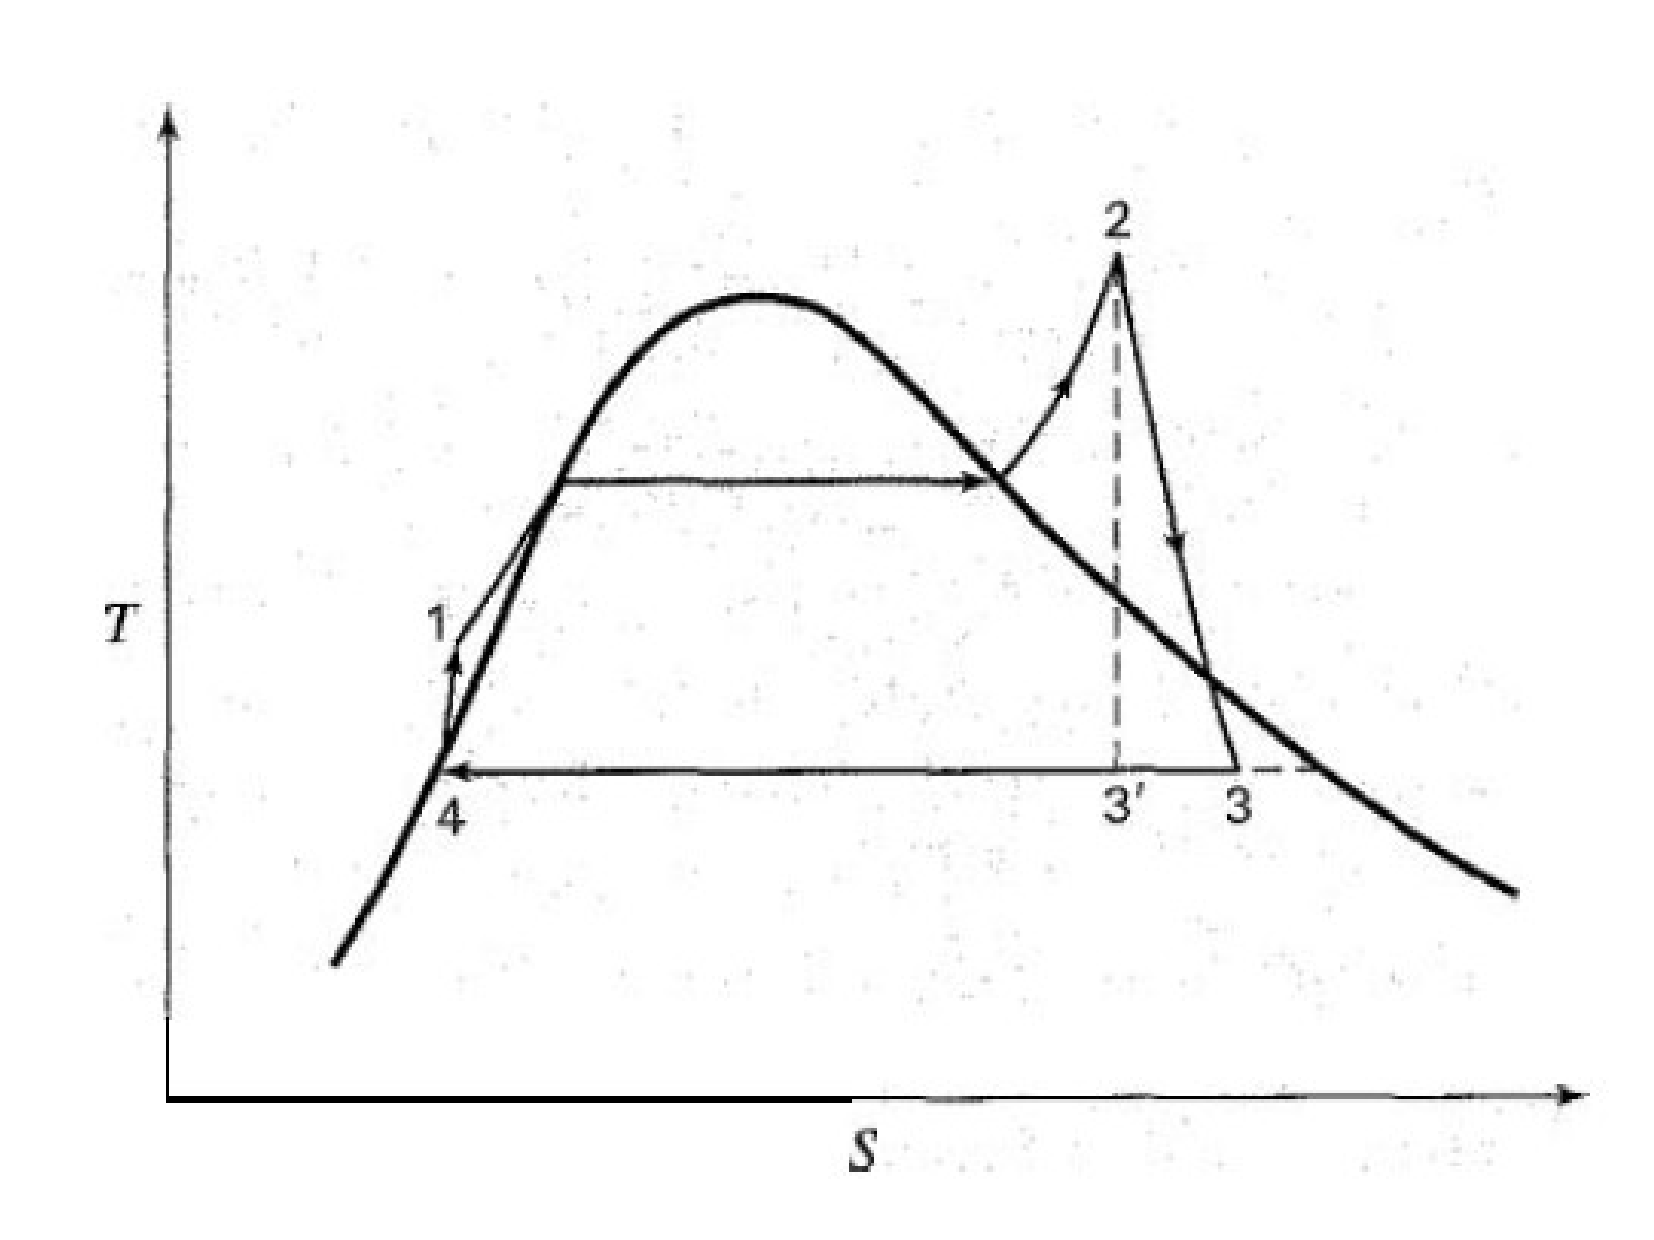
\includegraphics[width=12.cm,clip]{./../../ThermalEngines/Pics/Generic_Steam_Cycle}
%    \end{center}
%    \caption{Generic steam power plant.}\label{GenericSteamPlant}
%     \end{figure}

%%%
%%% Example 12.25 (Rajput)
%%%
\item\label{P:example12_25} {\it A steam power plant operates with with regenerative and reheat arrangement cycles. Steam is supplied to the H.P. turbine (Fig. \ref{example12_25}a) at 80 bar and 470$^{o}$C.  For feed heating, a part of steam is extracted at 7 bar and remainder of the steam is reheated to 350$^{o}$C in a reheater and then expanded in L.P. turbine down to 0.035 bar. Determine: (a) amount of steam bled-off for feed heating; (b) amount of steam supplied to L.P. turbine; (c) heat supplied to the boiler and reheater; (d) cycle efficiency, and (e) power developed by the system. The steam supplied by the boiler is 50 kg/s.}
   \begin{figure}[h]
    \begin{center}
    \vbox{
     \hbox{\hspace{1cm}
      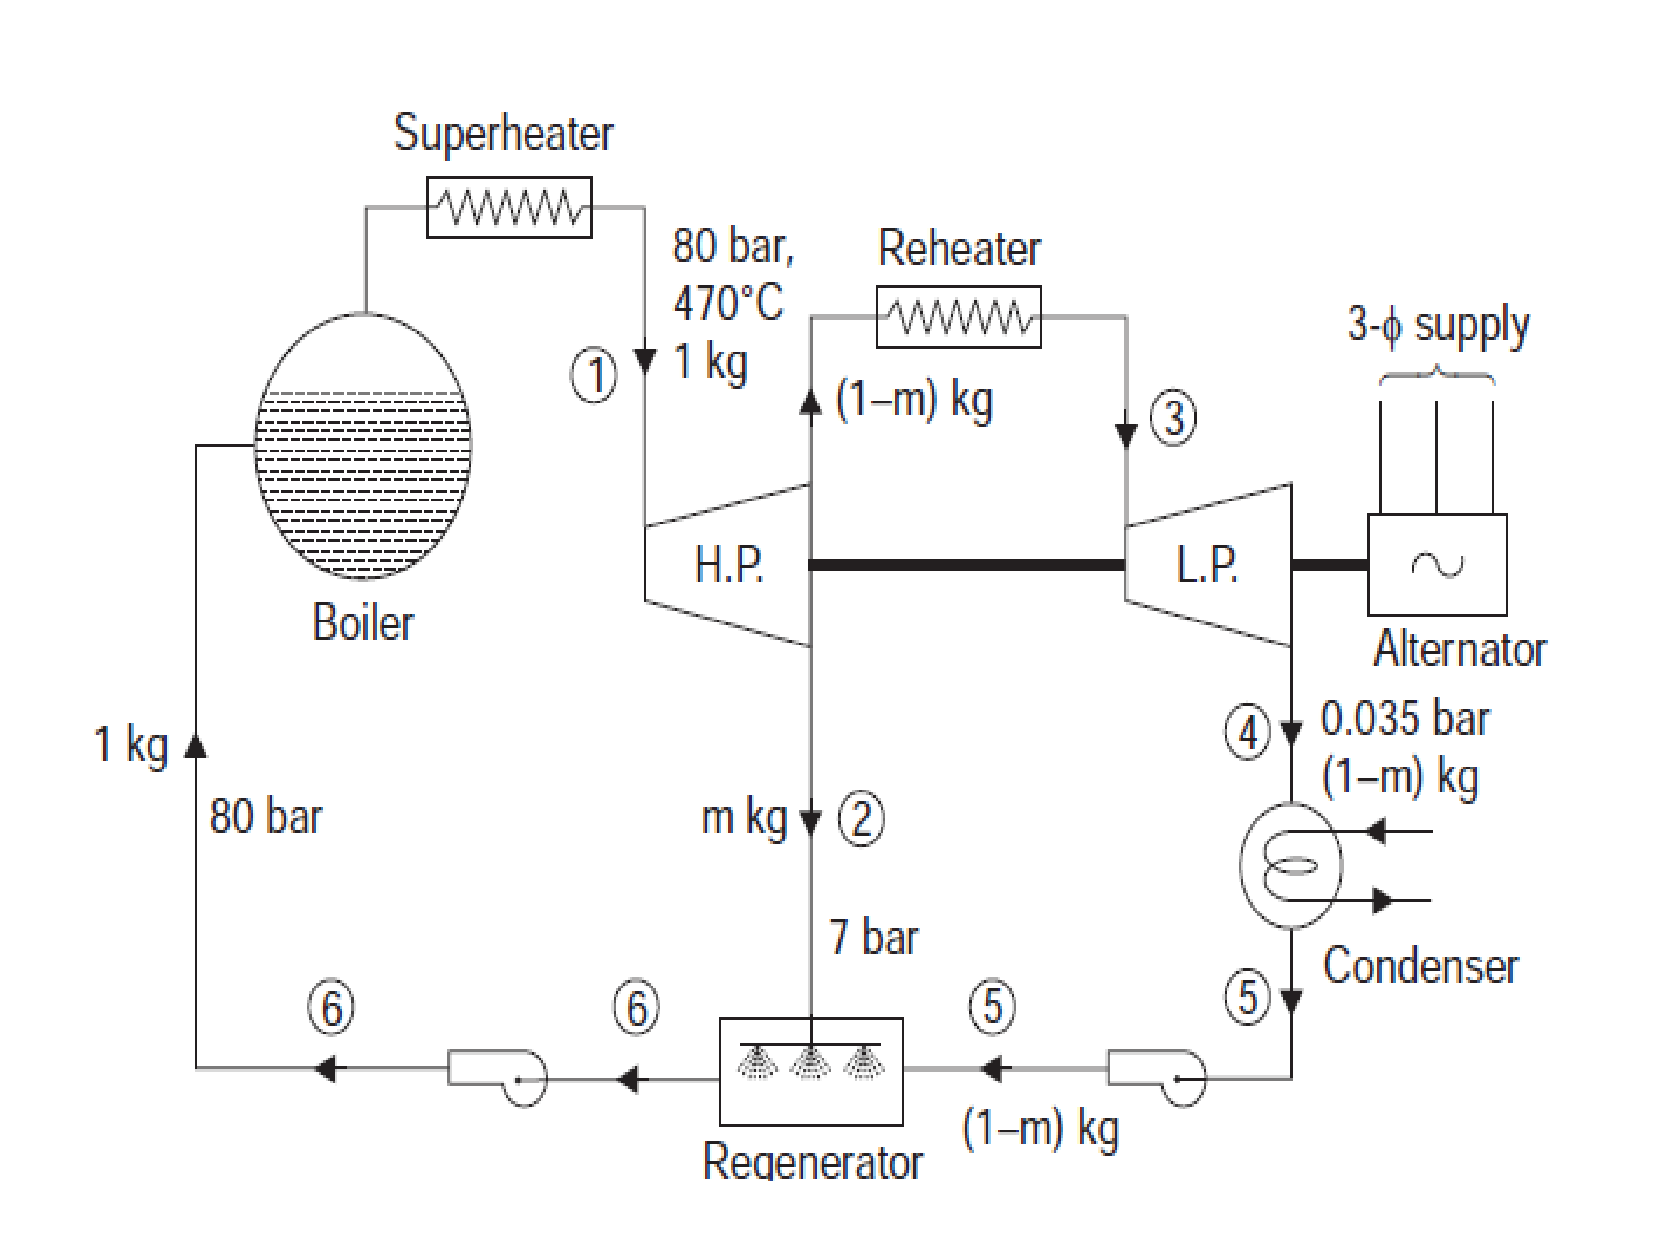
\includegraphics[width=12.cm,clip]{./../../ThermalEngines/Pics/Exemple12_25a_Rajput}}
     \hbox{\hspace{7.5cm}(a)}
     \hbox{\hspace{1.cm}
      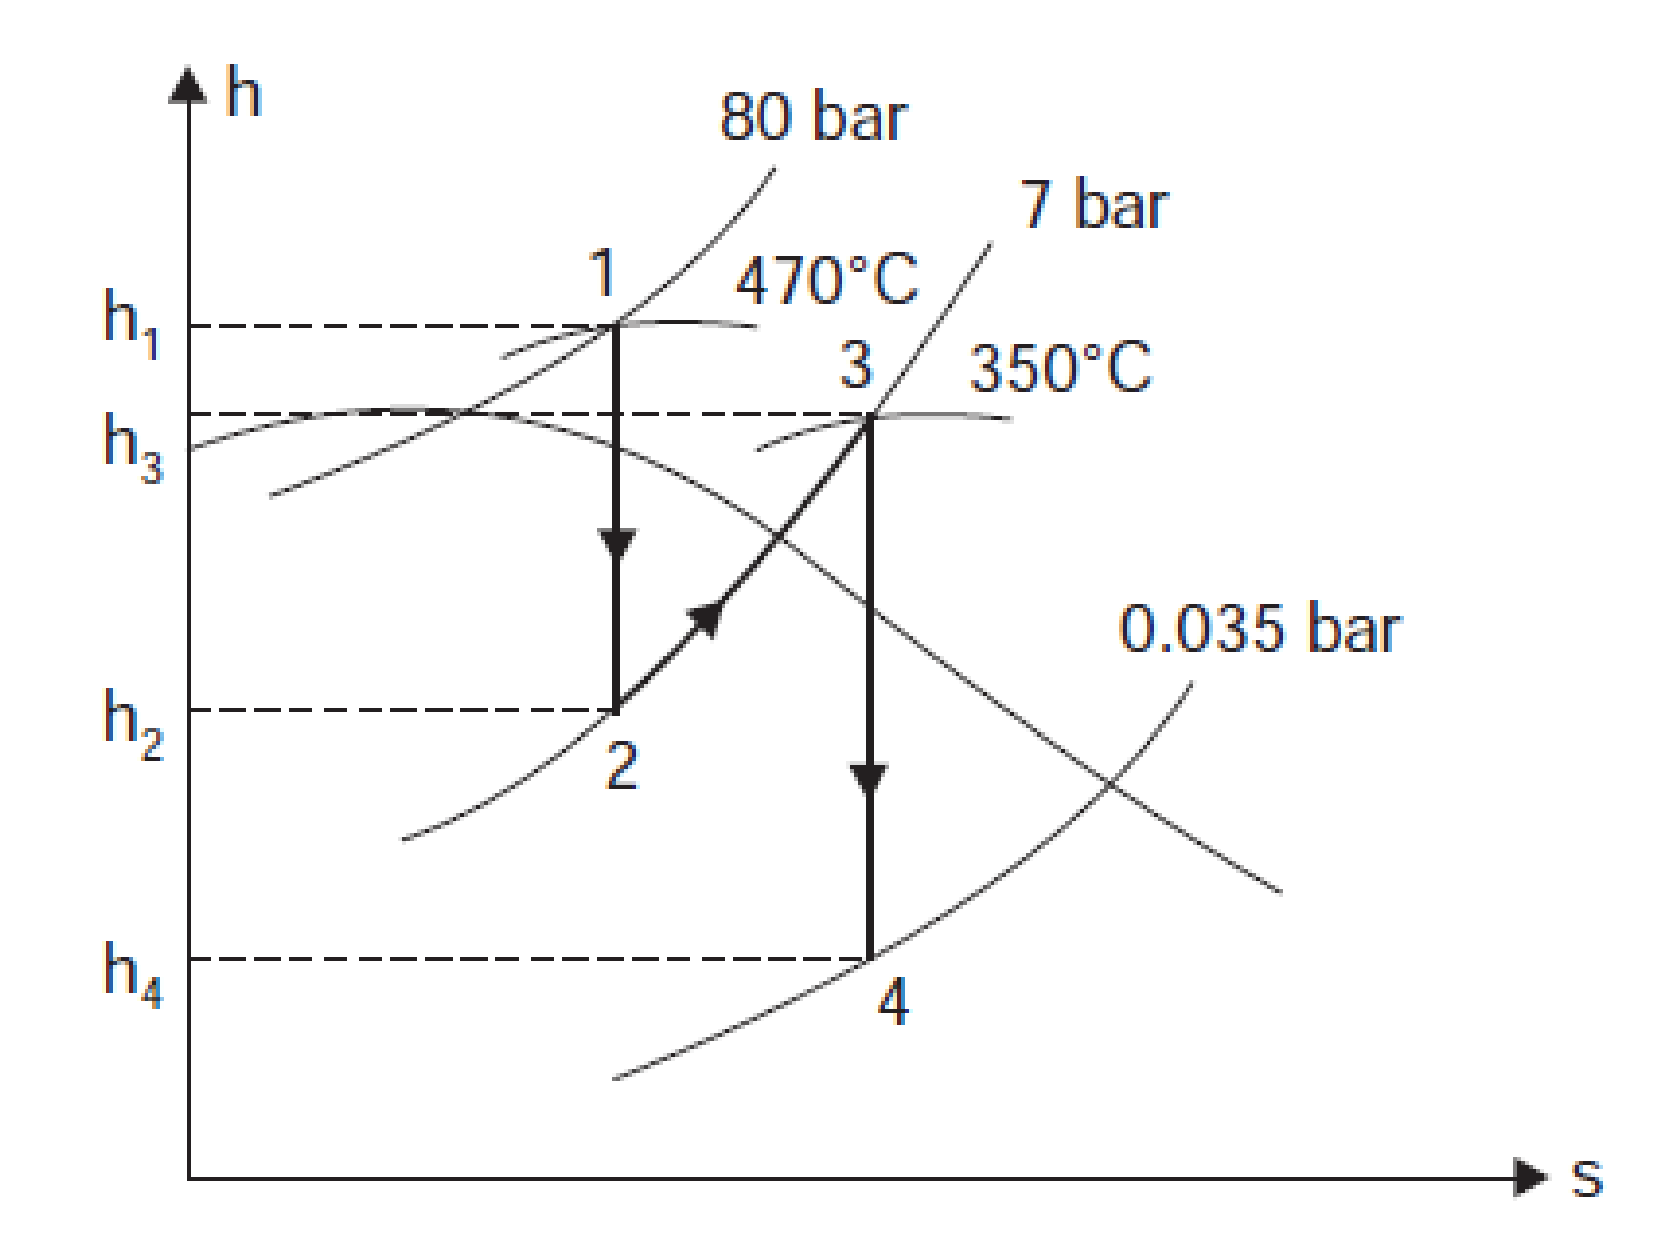
\includegraphics[width=12.cm,clip]{./../../ThermalEngines/Pics/Exemple12_25b_Rajput}
      }
     \hbox{\hspace{7.5cm}(b)}}
     \caption{Problem \ref{P:example12_25}: (a) Schematics and (b) $hs$ diagram of a steam power cycle.}
     \label{example12_25}
     \end{center}
   \end{figure}
 

%%%
%%% Problem 8.6 (Saphiro)
%%%
\item {\it Water is the working fluid in an ideal Rankine cycle. Saturated vapour enters the turbine at 16 MPa, and the condenser pressure is 8 kPa. The mass flow rate of steam entering in the turbine is 120 kg/s. Calculate:
\begin{enumerate}
\item the net power developed (in MW);
\item rate of heat transfer to the steam passing through the boiler (in MW);
\item thermal efficiency;
\item mass flow rate of the condenser cooling water (in kg/s(, if the cooling water undergoes a temperature increase of 18$^{o}$C with negligible pressure change in passing through the condenser.
\end{enumerate} 
}


%%%
%%% Problem 8.12 (Saphiro)
%%%
\item {\it A power plant based on the Rankine cycle is under development to provide a net power output of 10MW. Solar collectors are to be used to generate Refrigerant 22 vapour at 1.6MPa and 50$^{o}$C, for expansion through the turbine. Cooling water is available ar 20$^{o}$C. Specify he preliminary design of the cycle and estimate the thermal efficiency and the refrigerant and cooling water flow rates (in kg/s).}



%%%
%%% Problem 8.16 (Saphiro)
%%%
\item {\it Steam enters the turbine of a simple vapour power plant with a pressure of 10 MPa and temperature $T$, and expands adiabatically to 6 KPa. The isentropuc turbine efficiency is 85$\%$. Saturated liquid exits the condenser at 6KPa and the isentropic pump efficiency is 82$\%$.
\begin{enumerate}
\item For $T=580^{o}$C, determine the turbine exit quality and the cycle thermal efficiency;
\item Compute the same of (a) for $T=700^{o}$C.
\end{enumerate}
}





%%%
%%% Problem 8.6 (SM&VN)
%%%
%\item {\it A steam power plant employs two adiabatic turbines in series. Steam enters the first turbine at 650$^{o}\text{C}$ and 7000 kPa and discharges from the second turbine at 20 kPa. The system is designed for equal power outputs from the two turbines, based on a turbine efficiency of 78$\%$ for each turbine. Determine the temperature and pressure of the steam in its intermediate state between the two turbines. What is the overall efficiency of the two turbines together with respect to isentropic expansion of the steam from the initial to the final state? }

%%%
%%% Problem 8.14 (Saphiro)
%%%
%\item \label{P:problem_lava}{\it On the south coast of the island of Hawaii, lava flows continuously into the ocean. It is proposed to anchor a floating power plant off-shore of the lava flow that uses ammonia as the working fluid. The plant would exploit the temperature variation between the warm water near the surface at 130$^{o}$F and seawater at 50$^{o}$F from a depth of 500 ft to produce power. Figure \ref{problem_lava} shows the configuration and provides additional data. Using the properties of pure water for the seawater and modelling the power as a Rankine cycle, calculate: (a) the thermal efficiency; (b) the mass flow rate of ammonia (in kg/h) for a net output of 300 HP.}
%   \begin{figure}[h]
%    \begin{center}
%      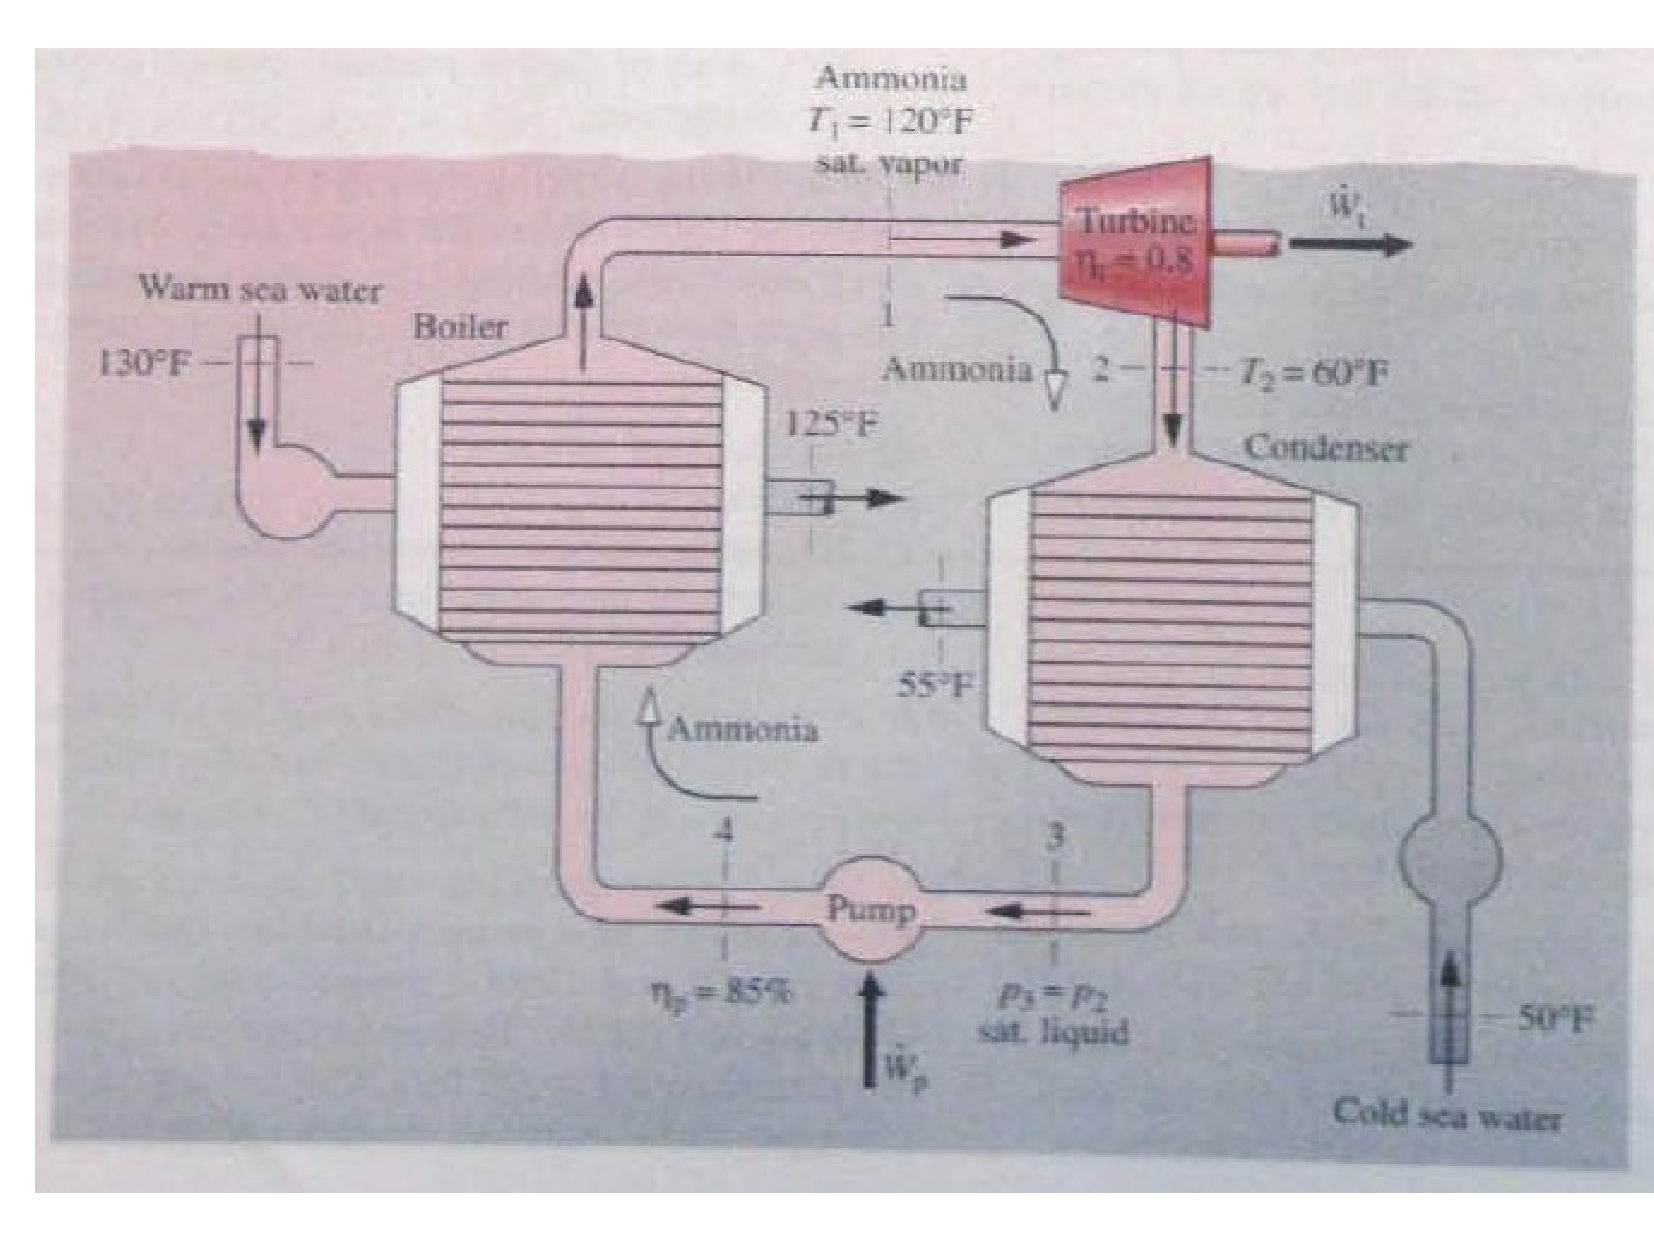
\includegraphics[width=12.cm,clip]{./../../ThermalEngines/Pics/LavaVolcanoPlant}
%     \caption{Problem \ref{P:problem_lava}: Schematics a steam power cycle.}
%     \label{problem_lava}
%     \end{center}
%   \end{figure}


%%%
%%% Problem 8.33 (Saphiro)
%%%
\item {\it Steam at 32 MPa and 520$^{o}$C enters the first stage of a supercritical reheat cycle including three turbine stages. Steam exiting the first-stage turbine at pressure $P$ is reheated at constant pressure to 440$^{o}$C, and steam exiting the second-stage turbine at 0.5 MPa is reheated at constant pressure to 360$^{o}$C.  Each turbine stage and the pump has an isentropic effciency of 85$\%$. The condenser pressure is at 8 kPa. For $P=4\;MPa$, determine the net work per unit mass of steam flowing (kJ/kg) and the thermal efficiency.}


%%%
%%% Problem 8.9 (SM&VN). \ref{example8_9})
%%%
\item \label{P:example8_9}{\it Steam power plant operating on a regenerative cycle, includes just one feedwater heater. Steam enters the turbine at 4500 kPa and 773.15 K and exhausts at 20 kPa. Steam for the feedwater heater is extracted from the turbine at 350 kPa, and in condensing raises the temperature of the feedwater to within 6 K of its condensation temperature at 350 kPa. If the turbine and pump efficiencies are both 0.78, what is the thermal efficiency of the cycle and what fraction of the steam entering the turbine is extracted for the feedwater heater?}



%\item \label{P:example8_9}{\it A steam power plant operating on a regenerative cycle (Fig. \ref{example8_9}), includes two feedwater heaters. Steam enters the turbine at 6500 kPa and 873.15 K and exhausts at 20 kPa. Steam for the feedwater heaters is extracted from the turbine at pressures such that the feedwater is heated to 463.15 K in two equal increments of temperature rise, with 5 K approaches to the steam-condensation temperature in each feedwater heater. If the turbine and pump efficiencies are both 0.80, what is the thermal efficiency of the cycle and what fraction of the steam entering the turbine is extracted for each feedwater heater? }


%\item \label{P:example8_10}{\it A power plant operating on heat recovered from the exhaust gases of internal combustion engines uses isobutane as the working medium in a modified Rankine cycle in which the upper pressure level is above the critical pressure of isobutane. Thus the isobutane does not undergo a change of phase as it absorbs heat prior to its entry into the turbine. Isobutane vapour is heated at 4800 kPa to 533.15 K, and enters the turbine as a supercritical fluid at these conditions. Isentropic expansion in the turbine produces a superheated vapour at 450 kPa, which is cooled and condensed at constant pressure. The resulting saturated liquid enters the pump for return to the heater. If the power output of the modified Rankine cycle is 1000 kW, what is the isobutane flow rate, the heat-transfer rates in the heater and condenser, and the thermal efficiency of the cycle? The vapour pressure of isobutane is given by
%\begin{displaymath}
%\ln\left(P^{\text{sat}}\right) = 1 - \frc{2606.775}{T+0.918}\;\;\;\text{with}\;\;\;\left[P^{\text{sat}}\right]=\text{kPa}\;\;\;\text{and}\;\;\;\left[T\right]=\text{K}
%\end{displaymath}
%Also, the enthalpy of the liquid flows can be obtained from
%\begin{displaymath}
%\Delta H = C_{p}\Delta T + V\left(1-\beta T\right)\Delta P
%\end{displaymath} 
%where
%\begin{displaymath}
%\beta=\frc{1}{V}\left(\frc{\partial V}{\partial T}\right)_{P}
%\end{displaymath}
%is the volume expansivity of fluid.
%}


   %\begin{figure}[h]
   % \begin{center}
   %   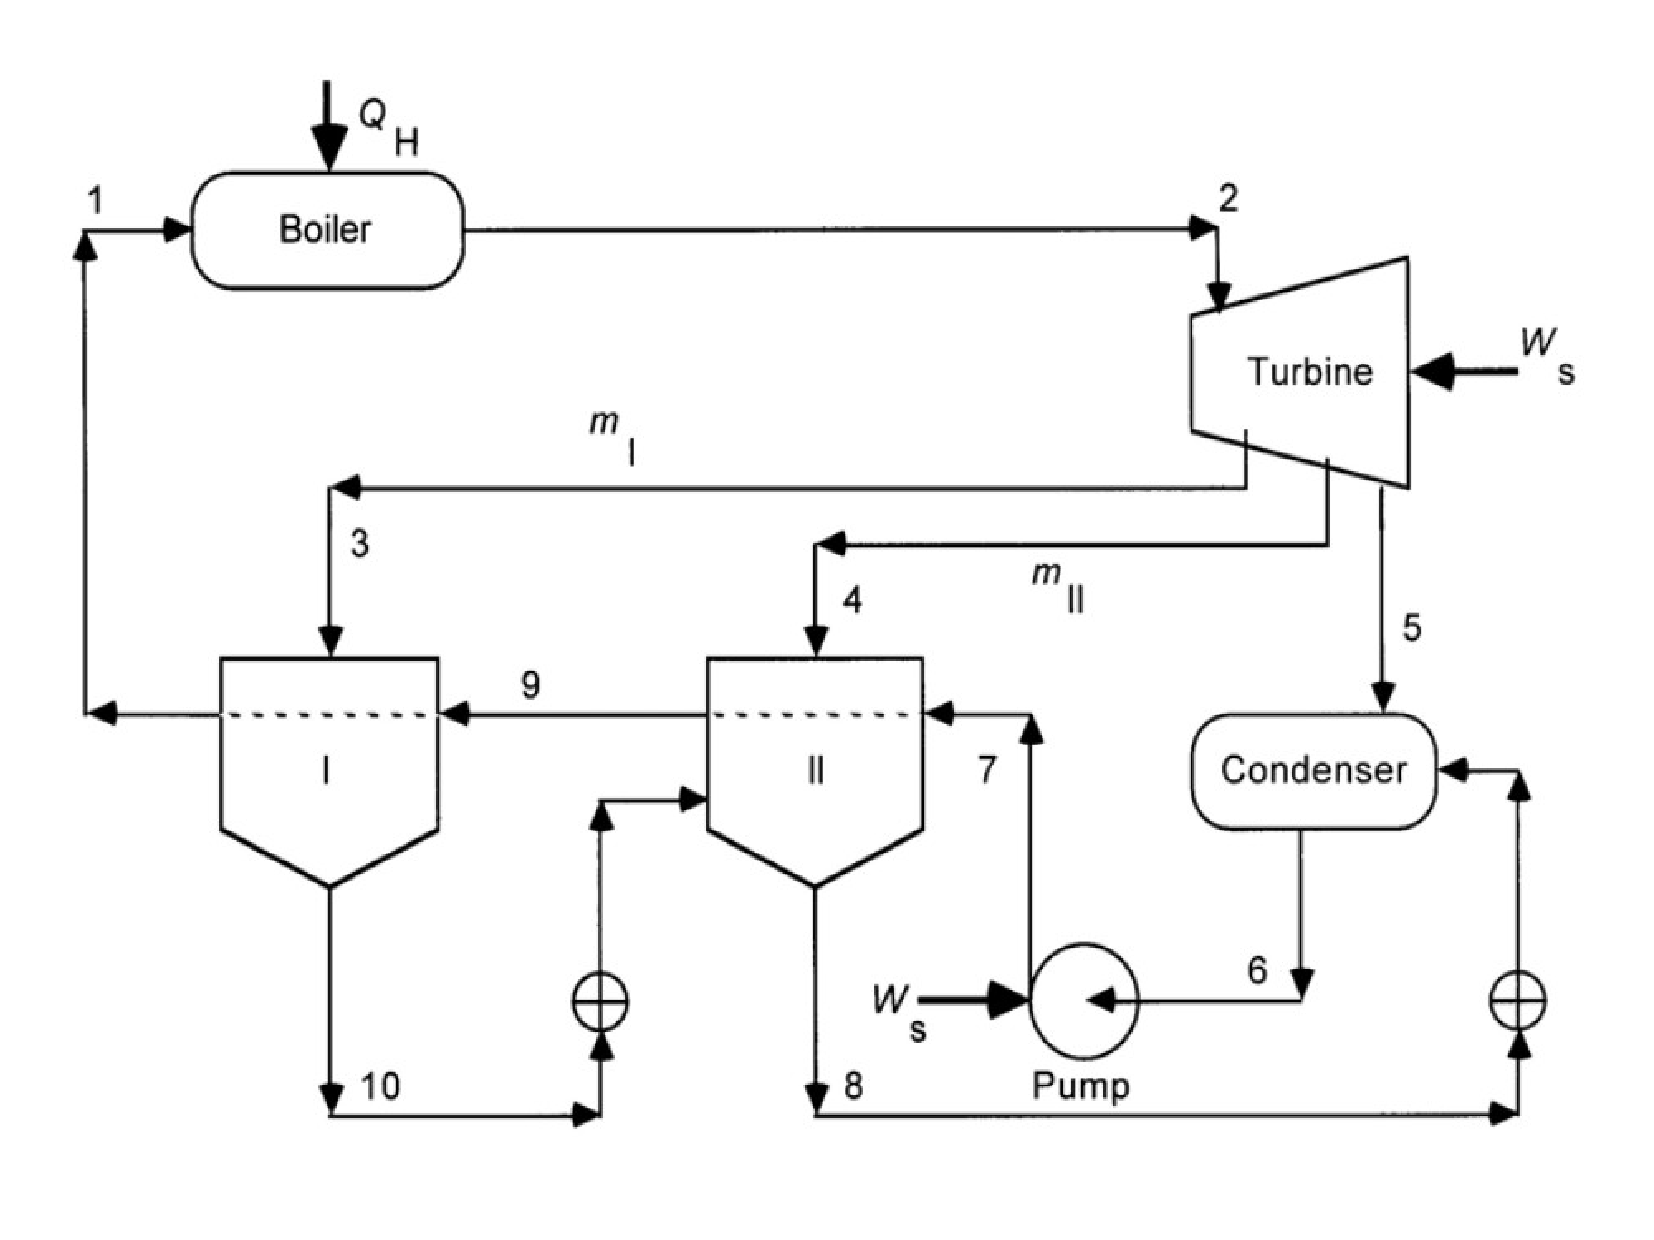
\includegraphics[width=12.cm,clip]{./../../ThermalEngines/Pics/Example_SMVN_8_9}
   %  \caption{Problem \ref{P:example8_9}: Schematics modified Rankine power cycle.}
   %  \label{example8_9}
   %  \end{center}
   %\end{figure}
 


%%%
%%% Problem 8.10 (SM&VN)
%%%
%\item {\it A power plant operating on heat from a geothermal source uses isobutane as the working medium in a Rankine cycle (Fig.\ref{GenericSteamPlant}). Isobutane is heated at 4.8 MPa (a pressure just below its critical pressure) to a temperature of 533.15 K, at which conditions it enters the turbine. Isentropic expansion in the turbine produces superheated vapour at 450 kPa, which is cooled and condensed to saturated liquid and pumped to the heater/boiler. If the flow rate of isobutane is 75 kg/s, what is the power output of the Rankine cycle and what are the heat-transfer rates in the heater/boiler and cooler/condenser? What is the thermal efficiency of the cycle? Repeat these calculations for a cycle in which the turbine and pump each have an efficiency of 80$\%$. The vapour pressure of isobutane is given in Problem \ref{P:example8_9}.}



\end{enumerate}




\pagebreak

\subsection{Gas Power Systems}

\begin{enumerate}

%%%
%%% Carnot: Example 13.4 (Rajput)
%%%
\item {\it A reversible engine converts one-sixth of the heat input into work. When the temperature of the sink is reduced by 70$^{\text{ o}}$C, its efficiency is doubled. Determine the temperature of the source and the sink.}

Let's first stablish that $T_{1}\text{ and }T_{2}\;\left[\text{K}\right]$ are the source and sink temperatures, respectively. For a {\bf reversible engine}, converting 1/6 of the heat into work means
\begin{displaymath}
\frc{T_{1}-T_{2}}{T_{1}}=\frc{1}{6} \;\;\; \Longrightarrow \;\;\; \textcolor{blue}{T_{1}=1.2T_{2}}
\end{displaymath}
Now if the sink temperature is reduced to {\it 70$^{\text{ o}}$C = 343.15 K}, ie, $T_{2}^{\prime}=T_{2}-343.15$ then the efficiency of the cycle is doubled
\begin{eqnarray}
&& \frc{T_{1}-T_{2}^{\prime}}{T_{1}}=2\times\frc{1}{6} \nonumber \\
&& 2T_{1}=3T_{2}-1029.45\;\;\Longrightarrow\;\;T_{2}=1715\text{ K and }T_{1}=2058.90\text{ k}\nonumber
\end{eqnarray}

%%%
%%% Carnot: Example 13.6 (Rajput)
%%%
\item {\it An ideal engine operates on the Carnot cycle using a perfects gas as the working fluid. The ratio of the greatest to the least volume is fixed as $x : 1$, the lower temperature of the cycle is also fixed, but the volume compression ratio $r$ of the reversible adiabatic compression is variable. The ratio of the specific heats is $\gamma$. Show that if the work done in the cycle is a maximum then,
\begin{displaymath}
  \left(\gamma-1\right)\ln\frc{x}{r}+\frc{1}{r^{\gamma-1}}-1=0
\end{displaymath}
}

%%%
%%% Otto: Example 13.9 (Rajput)
%%%
\item {\it The minimum pressure and temperature in an Otto cycle are 100 kPa and 27 $^{\text{ o}}$C. The amount of heat added to the air per cycle is 1500 kJ/kg. Calculate:
\begin{enumerate}
\item Pressures and temperatures at all stages of the air standard Otto cycle;
\item Specific  work and thermal efficiency of the cycle for a compression ratio of 8 : 1.
\end{enumerate}
}
Assuming an isentropic compression stage 1--2 and an isentropic expansion stage 3--4 with a compression ratio $V_{1}/V_{2}= 8$. Initial temperature of 300.15 K and pressure of 100 kPa.
\begin{itemize}
%
\item {\it adiabatic compression (1--2):}
\begin{displaymath}
  \frc{T_{2}}{T_{1}}=\left(\frc{V_{1}}{V_{2}}\right)^{\gamma-1}=r^{\gamma-1}=8^{1.4-1}=2.297\;\;\Longrightarrow\;\;T_{2}=689.10\text{ K}
\end{displaymath}
and
\begin{displaymath}
\frc{P_{1}}{P_{2}}=\left(\frc{V_{1}}{V_{2}}\right)^{\gamma}=18.379\;\Longrightarrow P_{2}=18.379\text{ bar}
\end{displaymath}

\item {\it constant volume (2--3):} heat added: $C_{v}\left(T_{3}-T_{2}\right)=1500\Longrightarrow T_{3}=2772.4\text{ K}$ and 
\begin{displaymath}
\frc{P_{2}}{T_{2}}=\frc{P_{3}}{T_{3}}\Longrightarrow P_{3}=73.94\text{ bar}
\end{displaymath}

\item {\it adiabatic expansion (3--4):}
\begin{displaymath}
\frc{T_{3}}{T_{4}}=\left(\frc{V_{4}}{V_{3}}\right)^{\gamma-1}=r^{\gamma-1}\;\Longrightarrow T_{4}=1206.9\text{ K}
\end{displaymath}
and
\begin{displaymath}
P_{3}V_{3}^{\gamma}=P_{4}V_{4}^{\gamma}\;\Longrightarrow P_{4}=4.023\text{ bar}
\end{displaymath}

\item {\it Specific work} = heat added - heat rejected
\begin{displaymath}
W= C_{v}\left(T_{3}-T_{2}\right)-C_{v}\left(T_{4}-T_{1}\right)=847\text{ kJ/kg}
\end{displaymath}

\item {\it Thermal efficiency:}
\begin{displaymath}
\eta_{\text{Otto}}=1- \frc{1}{r^{\gamma-1}} = 0.5647
\end{displaymath}
%
\end{itemize}


%%%
%%% Otto: Example 13.10 (Rajput)
%%%
\item {\it An ideal Otto cycle has a volumetric compression ratio of 6, the lowest cycle pressure of 0.1 MPa and operates between temperature limits of 300.15 and 1842.15 K.
\begin{enumerate}
\item \label{a}Calculate the temperature and pressure after the isentropic expansion;
\item Since the values in (\ref{a}) are well above the lowest cycle operating conditions, the expansion process was allowed to continue down to a pressure of 0.1 MPa. Which process is required to complete the cycle ? 
\item  Determine the percentage in which the cycle efficiency has improved.
\end{enumerate}
}

%%%
%%% Otto: Example 13.12 (Rajput)
%%%
%\item {\it In a constant volume Otto cycle, the pressure at the end of compression stroke is 15 times that at the start. The temperature of air at the beginning of compression is 38 $^{\text{ o}}$C and maximum temperature attained in the cycle is 1950 $^{\text{ o}}$C. Calculate: (i) compression ratio; (ii) thermal efficiency of the cycle and (iii) work done.}


%%%
%%% Diesel: Example 13.22 (Rajput)
%%%
\item {\it The volume ratios of compression and expansion for a diesel engine are 15.3 and 7.5, respectively. The pressure and temperature at the beginning of the compression are 1 bar and 27 $^{\text{ o}}$C. Assuming an ideal engine, determine the (a) MEP, (b) ratio of maximum pressure to MEP and (c) cycle efficiency. Also find the fuel consumption per kWh if the indicated thermal efficiency is 0.5 of ideal efficiency, mechanical efficiency is 0.8 and the calorific value of oil 42000 kJ/kg. }


%%%
%%% Dual: Prob 9.33 (Saphiro) 
%%%
%\item {\it An air-standard dual cycle has a compression ratio of 9. At the beginning of compression, $P_{1}=100\text{ kPa}$, $T_{1}=300\text{ K}$ and $V_{1}=14\text{ liters}$. The heat addition is 22.7 KJ with one-half added at constant volume and one-half added at constant pressure. Determine: (a) the temperatures at the end of each heat addition process; (b) the net work of the cycle per unit mass of air; (c) the thermal efficiency and; (d) MEP.}

\end{enumerate}


\setcounter{page}{1}
\pagenumbering{roman}
\begin{appendix}

\section{Introduction to Partial Differentiation}
Eight properties of a system -- pressure ({\it P}), volume ({\it V}), temperature ({\it T}), internal energy ({\it u}), enthalpy ({\it h}), entropy ({\it s}), Helmholtz free energy ({\it f}) and Gibbs free energy ({\it g}) have been introduced in EG2004 (Fluid Mechanics and Thermodynamics) and EG3020 (Process Thermodynamics). {\it h}, {\it f} and {\it g} are sometimes referred to as thermodynamic potentials. Both {\it f} and {\it g} are extremely important when considering chemical reactions (e.g., combustion) and processes involving phase change (e.g., water/steam industrial systems, atmospheric and crystallisation processes etc).

From the aforementioned (eight) properties, only pressure, temperature and volume can be directly measurable. Therefore it is convenient to introduce other combination of properties which are relatively easily measurable and which, along with {\it P}, {\it T} and {\it V}, enable the values of the remaining properties to be determined. These combinations of properties are commonly referred as {\it thermodynamic gradients} -- i.e., they are defined as the rate of change of one property with another while a third is kept constant.

\medskip

Let's consider three variables $x$, $y$ and $z$, and their functional relationship, $f\left(x,y,z\right)=0$ with $x=x(y,z)$, $y=y(x,z)$ and $z=z(x,y)$.  The intrinsic relationship of the differential dependent variable $x=x(y,z)$ in relation to the independent variables $y$ and $z$ can be represented as
\begin{equation}
dx = \left(\frc{\partial x}{\partial y}\right)_{z}dy + \left(\frc{\partial x}{\partial z}\right)_{y}dz
\label{exact_diff_dx}
\end{equation}
\noindent
in which $dx$ is the exact differential. Renaming $M=\left(\frc{\partial x}{\partial y}\right)_{z}$ and $N=\left(\frc{\partial x}{\partial z}\right)_{y}$, and Eqn. \ref{exact_diff_dx} can be rewritten as,
\begin{equation}
dx = Mdy + Ndz \label{diff1}
\end{equation}
\noindent
The partial differentiation of $M$ and $N$ with respect to $z$ and $y$, respectively, leads to,
\begin{equation}
  \frc{\partial M}{\partial z}=\frc{\partial^{2} x}{\partial y \partial z} \;\;\;\text{and}\;\;\; \frc{\partial N}{\partial y}=\frc{\partial^{2} x}{\partial z \partial y} \;\; \Longleftrightarrow \;\;  \frc{\partial M}{\partial z}=\frc{\partial N}{\partial y} \label{diff2}
\end{equation}
\noindent
Similarly for $y=y(x,z)$ and $z=z(x,y)$, 
\begin{eqnarray}
  dy = \left(\frc{\partial y}{\partial x}\right)_{z}dx + \left(\frc{\partial y}{\partial z}\right)_{x}dz \nonumber \\
  dz = \left(\frc{\partial z}{\partial x}\right)_{y}dx + \left(\frc{\partial z}{\partial y}\right)_{x}dy \nonumber
\end{eqnarray}
\noindent
Replacing $dz$ in $dy$ above,
\begin{eqnarray}
dy &=& \left(\frc{\partial y}{\partial x}\right)_{z}dx +  \left(\frc{\partial y}{\partial z}\right)_{x} \left[ \left(\frc{\partial z}{\partial x}\right)_{y}dx + \left(\frc{\partial z}{\partial y}\right)_{x}dy \right] \nonumber \\
%
  &=& \left[ \left(\frc{\partial y}{\partial x}\right)_{z} + \left(\frc{\partial y}{\partial z}\right)_{x} \left(\frc{\partial z}{\partial x}\right)_{y} \right]dx + dy \nonumber 
\end{eqnarray}
\noindent
Clearly, the term in the square-brackets vanishes,
\begin{eqnarray}
&& \left(\frc{\partial y}{\partial x}\right)_{z} + \left(\frc{\partial y}{\partial z}\right)_{x} \left(\frc{\partial z}{\partial x}\right)_{y}  = 0 \nonumber \\
%
&& \left(\frc{\partial y}{\partial z}\right)_{x} \left(\frc{\partial z}{\partial x}\right)_{y} =  -\left(\frc{\partial y}{\partial x}\right)_{z} \nonumber \\
&&  \left(\frc{\partial x}{\partial y}\right)_{z} \left(\frc{\partial z}{\partial x}\right)_{y} \left(\frc{\partial y}{\partial z}\right)_{x} = -1 \label{diff3}
\end{eqnarray}
\noindent
Replacing $x$, $y$ and $z$ by $P$, $V$ and $T$,
\begin{equation}
\left(\frc{\partial P}{\partial V}\right)_{T} = \left(\frc{\partial T}{\partial P}\right)_{V} = \left(\frc{\partial V}{\partial T}\right)_{P} = -1
\end{equation}

\section{Thermodynamic Relations}

From the Course Notes we saw that the First Law applied to a closed system in a reversible process states that,
\begin{equation}
dQ= du + PdV, \label{firstlaw_simplified}
\end{equation}
\noindent
and the Second Law,
\begin{equation}
ds=\left(\frc{dQ}{T}\right)_{\text{rev}}
\end{equation}
\noindent
we can combine these equations to obtain
\begin{equation}
du = - PdV + Tds \label{gibbs_eqn0}
\end{equation}
We can similarly derive the equations for enthalpy, free Gibbs and free Helmholtz energy equations as
\begin{eqnarray}
&& dh = Tds + VdP \label{enthalpy_eqn} \\
&& df = -PdV - sdT \label{helmholtz_eqn} \\
&& dg = -VdP -sdT \label{gibbs_eqn}
\end{eqnarray}

\noindent
As $du$, $dh$, $df$ and $dg$ are exact differentials, we can express them as the following set of chain rule -based differentials,
\begin{eqnarray}
du = \left(\frc{\partial u}{\partial  s}\right)_{V}ds + \left(\frc{\partial u}{\partial V}\right)_{s}dV \nonumber \\
%
dh = \left(\frc{\partial h}{\partial  s}\right)_{P}ds + \left(\frc{\partial h}{\partial P}\right)_{s}dP \nonumber \\
%
df = \left(\frc{\partial f}{\partial  V}\right)_{T}dV + \left(\frc{\partial f}{\partial T}\right)_{V}dT \nonumber \\
%
dg = \left(\frc{\partial g}{\partial  P}\right)_{T}dP + \left(\frc{\partial g}{\partial T}\right)_{P}dT \nonumber \\
\end{eqnarray}


\section{Maxwell Relations}

Comparing the Gibbs equation (\ref{gibbs_eqn0}) with Eqn. \ref{diff1} for $dx$,
\begin{displaymath}
du = -PdV +Tds \;\;\;\;\;\text{and}\;\;\;\;\; dx = Mdy + Ndz 
\end{displaymath}
We can easily notice the mathematical equivalences,
\begin{displaymath}
x\Longrightarrow u, \;\; y\Longrightarrow V, \;\; z\Longrightarrow s, \;\; M\Longrightarrow -P, \;\; N\Longrightarrow T
\end{displaymath}
\noindent
With the analogy of $x=x(y,z)$ and $u=u(V,s)$, Eqn. \ref{diff2} leads to,
\begin{equation}
-\left(\frc{\partial P}{\partial s}\right)_{V} = \left(\frac{\partial T}{\partial V}\right)_{s}, \label{maxwell_rel1} 
\end{equation}
\noindent
$\left(\frc{\partial u}{\partial V}\right)_{s} = -P$ and $\left(\frc{\partial u}{\partial s}\right)_{V}=T$.  Eqn. \ref{maxwell_rel1} is known as a {\it Maxwell relation}. Similar relations can be obtained from the remaining fundamental thermodynamics equations -- Eqns. \ref{enthalpy_eqn}-\ref{gibbs_eqn} leading to the whole set of {\it Maxwell relations}:
\begin{eqnarray}
%
 \left(\frac{\partial T}{\partial V}\right)_{s} &=& -\left(\frc{\partial P}{\partial s}\right)_{V} \nonumber \\
%
 \left(\frc{\partial T}{\partial P}\right)_{s} &=& \left(\frac{\partial V}{\partial s}\right)_{P} \label{maxwell_rel2} \\
%
 \left(\frc{\partial P}{\partial T}\right)_{V} &=& \left(\frac{\partial s}{\partial V}\right)_{T} \label{maxwell_rel3} \\
%
  \left(\frac{\partial V}{\partial T}\right)_{P} &=& -\left(\frc{\partial s}{\partial P}\right)_{T} \label{maxwell_rel4} 
\end{eqnarray}
\noindent
with,
\begin{eqnarray}
%
\left(\frc{\partial u}{\partial s}\right)_{V} & =  T  = & \left(\frc{\partial h}{\partial s}\right)_{P} \label{maxwell_coef1} \\
%
\left(\frc{\partial u}{\partial V}\right)_{s} & = - P = & \left(\frc{\partial f}{\partial V}\right)_{T} \label{maxwell_coef2} \\
%
\left(\frc{\partial h}{\partial P}\right)_{s} & =  V =  & \left(\frc{\partial g}{\partial P}\right)_{T} \label{maxwell_coef3} \\
%
\left(\frc{\partial f}{\partial T}\right)_{V} & =  -s  = & \left(\frc{\partial g}{\partial T}\right)_{P} \label{maxwell_coef4}
%
\end{eqnarray}

Equations \ref{maxwell_rel1}-\ref{maxwell_coef4} do not refer to a process, but do express relations between properties which must be satisfied when any system is in a state of equilibrium.




\end{appendix}

\end{document}
